\documentclass[]{book}
\usepackage{lmodern}
\usepackage{amssymb,amsmath}
\usepackage{ifxetex,ifluatex}
\usepackage{fixltx2e} % provides \textsubscript
\ifnum 0\ifxetex 1\fi\ifluatex 1\fi=0 % if pdftex
  \usepackage[T1]{fontenc}
  \usepackage[utf8]{inputenc}
\else % if luatex or xelatex
  \ifxetex
    \usepackage{mathspec}
  \else
    \usepackage{fontspec}
  \fi
  \defaultfontfeatures{Ligatures=TeX,Scale=MatchLowercase}
\fi
% use upquote if available, for straight quotes in verbatim environments
\IfFileExists{upquote.sty}{\usepackage{upquote}}{}
% use microtype if available
\IfFileExists{microtype.sty}{%
\usepackage{microtype}
\UseMicrotypeSet[protrusion]{basicmath} % disable protrusion for tt fonts
}{}
\usepackage{hyperref}
\hypersetup{unicode=true,
            pdftitle={Incorporating Spatial Analysis into Agricultural Field Experiments.},
            pdfauthor={Julia Piaskowski},
            pdfborder={0 0 0},
            breaklinks=true}
\urlstyle{same}  % don't use monospace font for urls
\usepackage{natbib}
\bibliographystyle{apalike}
\usepackage{color}
\usepackage{fancyvrb}
\newcommand{\VerbBar}{|}
\newcommand{\VERB}{\Verb[commandchars=\\\{\}]}
\DefineVerbatimEnvironment{Highlighting}{Verbatim}{commandchars=\\\{\}}
% Add ',fontsize=\small' for more characters per line
\usepackage{framed}
\definecolor{shadecolor}{RGB}{248,248,248}
\newenvironment{Shaded}{\begin{snugshade}}{\end{snugshade}}
\newcommand{\AlertTok}[1]{\textcolor[rgb]{0.94,0.16,0.16}{#1}}
\newcommand{\AnnotationTok}[1]{\textcolor[rgb]{0.56,0.35,0.01}{\textbf{\textit{#1}}}}
\newcommand{\AttributeTok}[1]{\textcolor[rgb]{0.77,0.63,0.00}{#1}}
\newcommand{\BaseNTok}[1]{\textcolor[rgb]{0.00,0.00,0.81}{#1}}
\newcommand{\BuiltInTok}[1]{#1}
\newcommand{\CharTok}[1]{\textcolor[rgb]{0.31,0.60,0.02}{#1}}
\newcommand{\CommentTok}[1]{\textcolor[rgb]{0.56,0.35,0.01}{\textit{#1}}}
\newcommand{\CommentVarTok}[1]{\textcolor[rgb]{0.56,0.35,0.01}{\textbf{\textit{#1}}}}
\newcommand{\ConstantTok}[1]{\textcolor[rgb]{0.00,0.00,0.00}{#1}}
\newcommand{\ControlFlowTok}[1]{\textcolor[rgb]{0.13,0.29,0.53}{\textbf{#1}}}
\newcommand{\DataTypeTok}[1]{\textcolor[rgb]{0.13,0.29,0.53}{#1}}
\newcommand{\DecValTok}[1]{\textcolor[rgb]{0.00,0.00,0.81}{#1}}
\newcommand{\DocumentationTok}[1]{\textcolor[rgb]{0.56,0.35,0.01}{\textbf{\textit{#1}}}}
\newcommand{\ErrorTok}[1]{\textcolor[rgb]{0.64,0.00,0.00}{\textbf{#1}}}
\newcommand{\ExtensionTok}[1]{#1}
\newcommand{\FloatTok}[1]{\textcolor[rgb]{0.00,0.00,0.81}{#1}}
\newcommand{\FunctionTok}[1]{\textcolor[rgb]{0.00,0.00,0.00}{#1}}
\newcommand{\ImportTok}[1]{#1}
\newcommand{\InformationTok}[1]{\textcolor[rgb]{0.56,0.35,0.01}{\textbf{\textit{#1}}}}
\newcommand{\KeywordTok}[1]{\textcolor[rgb]{0.13,0.29,0.53}{\textbf{#1}}}
\newcommand{\NormalTok}[1]{#1}
\newcommand{\OperatorTok}[1]{\textcolor[rgb]{0.81,0.36,0.00}{\textbf{#1}}}
\newcommand{\OtherTok}[1]{\textcolor[rgb]{0.56,0.35,0.01}{#1}}
\newcommand{\PreprocessorTok}[1]{\textcolor[rgb]{0.56,0.35,0.01}{\textit{#1}}}
\newcommand{\RegionMarkerTok}[1]{#1}
\newcommand{\SpecialCharTok}[1]{\textcolor[rgb]{0.00,0.00,0.00}{#1}}
\newcommand{\SpecialStringTok}[1]{\textcolor[rgb]{0.31,0.60,0.02}{#1}}
\newcommand{\StringTok}[1]{\textcolor[rgb]{0.31,0.60,0.02}{#1}}
\newcommand{\VariableTok}[1]{\textcolor[rgb]{0.00,0.00,0.00}{#1}}
\newcommand{\VerbatimStringTok}[1]{\textcolor[rgb]{0.31,0.60,0.02}{#1}}
\newcommand{\WarningTok}[1]{\textcolor[rgb]{0.56,0.35,0.01}{\textbf{\textit{#1}}}}
\usepackage{longtable,booktabs}
\usepackage{graphicx,grffile}
\makeatletter
\def\maxwidth{\ifdim\Gin@nat@width>\linewidth\linewidth\else\Gin@nat@width\fi}
\def\maxheight{\ifdim\Gin@nat@height>\textheight\textheight\else\Gin@nat@height\fi}
\makeatother
% Scale images if necessary, so that they will not overflow the page
% margins by default, and it is still possible to overwrite the defaults
% using explicit options in \includegraphics[width, height, ...]{}
\setkeys{Gin}{width=\maxwidth,height=\maxheight,keepaspectratio}
\IfFileExists{parskip.sty}{%
\usepackage{parskip}
}{% else
\setlength{\parindent}{0pt}
\setlength{\parskip}{6pt plus 2pt minus 1pt}
}
\setlength{\emergencystretch}{3em}  % prevent overfull lines
\providecommand{\tightlist}{%
  \setlength{\itemsep}{0pt}\setlength{\parskip}{0pt}}
\setcounter{secnumdepth}{5}
% Redefines (sub)paragraphs to behave more like sections
\ifx\paragraph\undefined\else
\let\oldparagraph\paragraph
\renewcommand{\paragraph}[1]{\oldparagraph{#1}\mbox{}}
\fi
\ifx\subparagraph\undefined\else
\let\oldsubparagraph\subparagraph
\renewcommand{\subparagraph}[1]{\oldsubparagraph{#1}\mbox{}}
\fi

%%% Use protect on footnotes to avoid problems with footnotes in titles
\let\rmarkdownfootnote\footnote%
\def\footnote{\protect\rmarkdownfootnote}

%%% Change title format to be more compact
\usepackage{titling}

% Create subtitle command for use in maketitle
\providecommand{\subtitle}[1]{
  \posttitle{
    \begin{center}\large#1\end{center}
    }
}

\setlength{\droptitle}{-2em}

  \title{Incorporating Spatial Analysis into Agricultural Field Experiments.}
    \pretitle{\vspace{\droptitle}\centering\huge}
  \posttitle{\par}
    \author{Julia Piaskowski}
    \preauthor{\centering\large\emph}
  \postauthor{\par}
      \predate{\centering\large\emph}
  \postdate{\par}
    \date{2019-07-26}

\usepackage{booktabs}

\begin{document}
\maketitle

{
\setcounter{tocdepth}{1}
\tableofcontents
}
\hypertarget{preface}{%
\chapter{Preface}\label{preface}}

\hypertarget{tutorial-goals}{%
\section{Tutorial goals}\label{tutorial-goals}}

To help people conducting planned agricultural field trials to understand and incorporate spatial variation routinely into analysis of field trials.

current resources are focused on geospatia appications - LANDSAT data across large area, point information on soils and geology, and other information that typiically requiresa a moderate to deep understanding of obht GIS tools and spatial analytica techniques.

Furthermore, there is not a comprehensive one-stop-shop for spatial analytical techniques for fied experiments that is also freely available.

\hypertarget{prerequisites}{%
\section{Prerequisites}\label{prerequisites}}

In order to run the scripts in this demonstration, you will to download R, avaiable free through the \href{}{Comprehensive R Archive Network}. While this is sufficient for running R scripts, You may also find it hepful to use RStudio, which provides a nice graphical user interface for R. RStudio can be downloaded \href{}{here}.

If you already have R installed, please make sure you have version 3.5.0 or newer.

This demonstration is not intended to provide instructions on general R usage. However, There are numerous web resources for learning the Basics of R:

\begin{itemize}
\item
\item
\item
\item
\end{itemize}

\hypertarget{packages-we-will-use}{%
\section{Packages we will use}\label{packages-we-will-use}}

\hypertarget{acknowledgements}{%
\section{Acknowledgements}\label{acknowledgements}}

\hypertarget{license}{%
\section{License}\label{license}}

\hypertarget{old-stuff}{%
\subsubsection{OLD STUFF}\label{old-stuff}}

This is a \emph{sample} book written in \textbf{Markdown}. You can use anything that Pandoc's Markdown supports, e.g., a math equation \(a^2 + b^2 = c^2\).

The \textbf{bookdown} package can be installed from CRAN or Github:

\begin{Shaded}
\begin{Highlighting}[]
\KeywordTok{install.packages}\NormalTok{(}\StringTok{"bookdown"}\NormalTok{)}
\CommentTok{# or the development version}
\CommentTok{# devtools::install_github("rstudio/bookdown")}
\end{Highlighting}
\end{Shaded}

Remember each Rmd file contains one and only one chapter, and a chapter is defined by the first-level heading \texttt{\#}.

To compile this example to PDF, you need XeLaTeX. You are recommended to install TinyTeX (which includes XeLaTeX): \url{https://yihui.name/tinytex/}.

\hypertarget{intro}{%
\chapter{Introduction}\label{intro}}

\hypertarget{why-care-about-spatial-variation}{%
\section{Why care about spatial variation?}\label{why-care-about-spatial-variation}}

Goal in this case is to understand and account for spatial variation. These are lattice data

\hypertarget{diagnosing-spatial-autocorrelation}{%
\section{Diagnosing spatial autocorrelation}\label{diagnosing-spatial-autocorrelation}}

Spatial correlation is similarity of plots that are close to one another. Larger spatial gradients need to modelled indpendently - perhaps through blocking.

\hypertarget{morans-i}{%
\subsection{Moran's I}\label{morans-i}}

Moran's I, sometimes called ``Global Moran's I'' is similar like a correlation coefficient. It is a test for correation between units (plots in our case).

\[ I = \frac{N}{W}\frac{\sum_i \sum_j w_{ij} (x_i - \bar{x})(x_j - \bar{x})}{\sum_i(x_i - \bar{x})^2} 
\qquad i \neq j\]

Where N is total number of spatial locations indexed by \(i\) and \(j\), x is the variable of interest, \(w_{ij}\) are a spatial weights between each \(i\) and \(j\), and W is the sum of all weights. The expected values of Moran's I is \(-1/(N-1)\). Values greater than that indicate positive spatial correlation (areas close to each other are similar), while values less than the expected Moran's I indicate dissimilarity as spatial distance between points decreases.

There are several options for defining adjacent neighbors and how to weight each neighbors's influence. The two common configuations for defininig neighbors are the rook and queen configurations. These are exactly what their chess analogy suggest: ``rook'' defines neighbhors in an row/column fashion, while ``queen'' defines nieghbors in a row/column configuation an also neighbors located diagonally at a 45 degree angle from the row/column neighbors. Determining this can be somewhat complicated when working with irregularly-placed data (e.g.~county seats), but is quite unambiguous for gridded data commonly seen in panned field experiments:

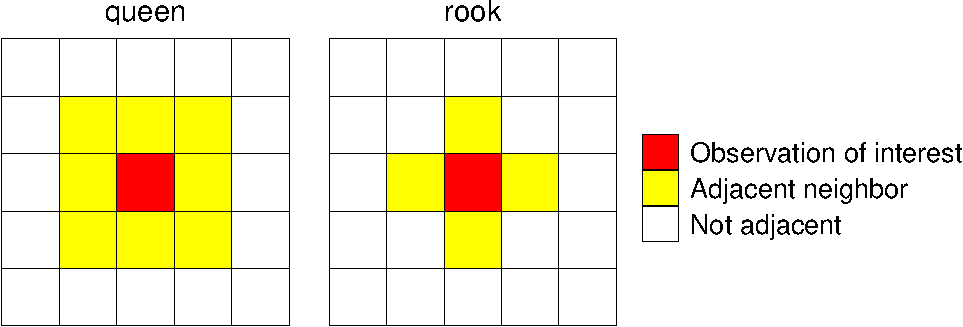
\includegraphics{Field-Trial-Spatial-Analysis-Guide_files/figure-latex/unnamed-chunk-3-1.pdf}

Another test for diagnosing spatial correlation is Geary's C:

\[ I = \frac{(N -1)}{2W}\frac{\sum_i \sum_j w_{ij} (x_i - x_j)^2}{\sum_i(x_i - \bar{x})^2} \qquad i \neq j\]

These terms have the same meaning in Moran's I. The expected value of Geary's C is 1. Values higher than 1 indicate positive spatial correlation and less than 1 indicate negative spatial correlation.

\hypertarget{empirical-variogram-semivariance}{%
\subsection{Empirical variogram \& semivariance}\label{empirical-variogram-semivariance}}

An empirical varigram is a visual tool for understanding how error terms are related to each other over spatial distance. It relies on semivariance (\(\gamma\)), a statistic expressing variance as a function of pairwise distances between data points at points \(i\) and \(j\).

\[\gamma(h) = \frac{1}{2|N(h)|}\sum_{N(h)}(x_i - x_j)^2\]

Semivariances are binned for distance intervals. The average values for semivariance and distance interval can be fit to correlated error models such a exponential, spherical, gaussian and Matér. How to dothis is explored further in section 2 of this guide.

Three important concepts of an empirical variogram are \emph{nugget}, \emph{sill} and \emph{range}

\begin{figure}
\centering
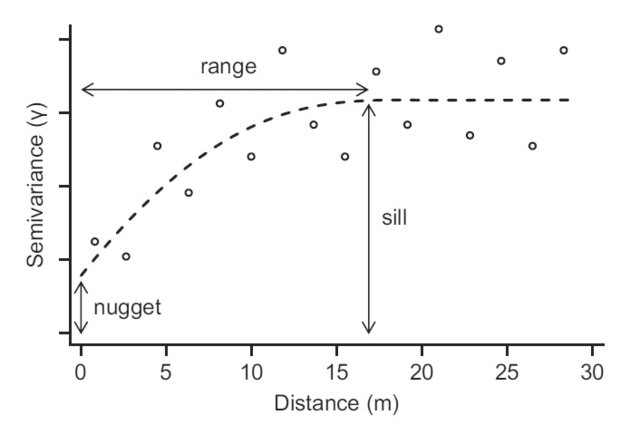
\includegraphics{img/Sadoti2014_spherical.jpg}
\caption{Example Empirical Variogram}
\end{figure}

\begin{itemize}
\tightlist
\item
  range = distance up to which is there is spatial correlation
\item
  sill = uncorrelated variance of the variable of interest
\item
  nugget = measurement error,short-distance spatial variance and other unaccounted for variance
\end{itemize}

2 other concepts:

\begin{itemize}
\tightlist
\item
  partial sill = sill - nugget
\item
  nugget effect = the nugget/sill ratio, interpreted opposite of \(r^2\)
\end{itemize}

\hypertarget{old-stuff-1}{%
\subsubsection{OLD STUFF}\label{old-stuff-1}}

You can label chapter and section titles using \texttt{\{\#label\}} after them, e.g., we can reference Chapter \ref{intro}. If you do not manually label them, there will be automatic labels anyway, e.g., Chapter \ref{methods}.

Figures and tables with captions will be placed in \texttt{figure} and \texttt{table} environments, respectively.

\begin{Shaded}
\begin{Highlighting}[]
\KeywordTok{par}\NormalTok{(}\DataTypeTok{mar =} \KeywordTok{c}\NormalTok{(}\DecValTok{4}\NormalTok{, }\DecValTok{4}\NormalTok{, }\FloatTok{.1}\NormalTok{, }\FloatTok{.1}\NormalTok{))}
\KeywordTok{plot}\NormalTok{(pressure, }\DataTypeTok{type =} \StringTok{'b'}\NormalTok{, }\DataTypeTok{pch =} \DecValTok{19}\NormalTok{)}
\end{Highlighting}
\end{Shaded}

\begin{figure}

{\centering 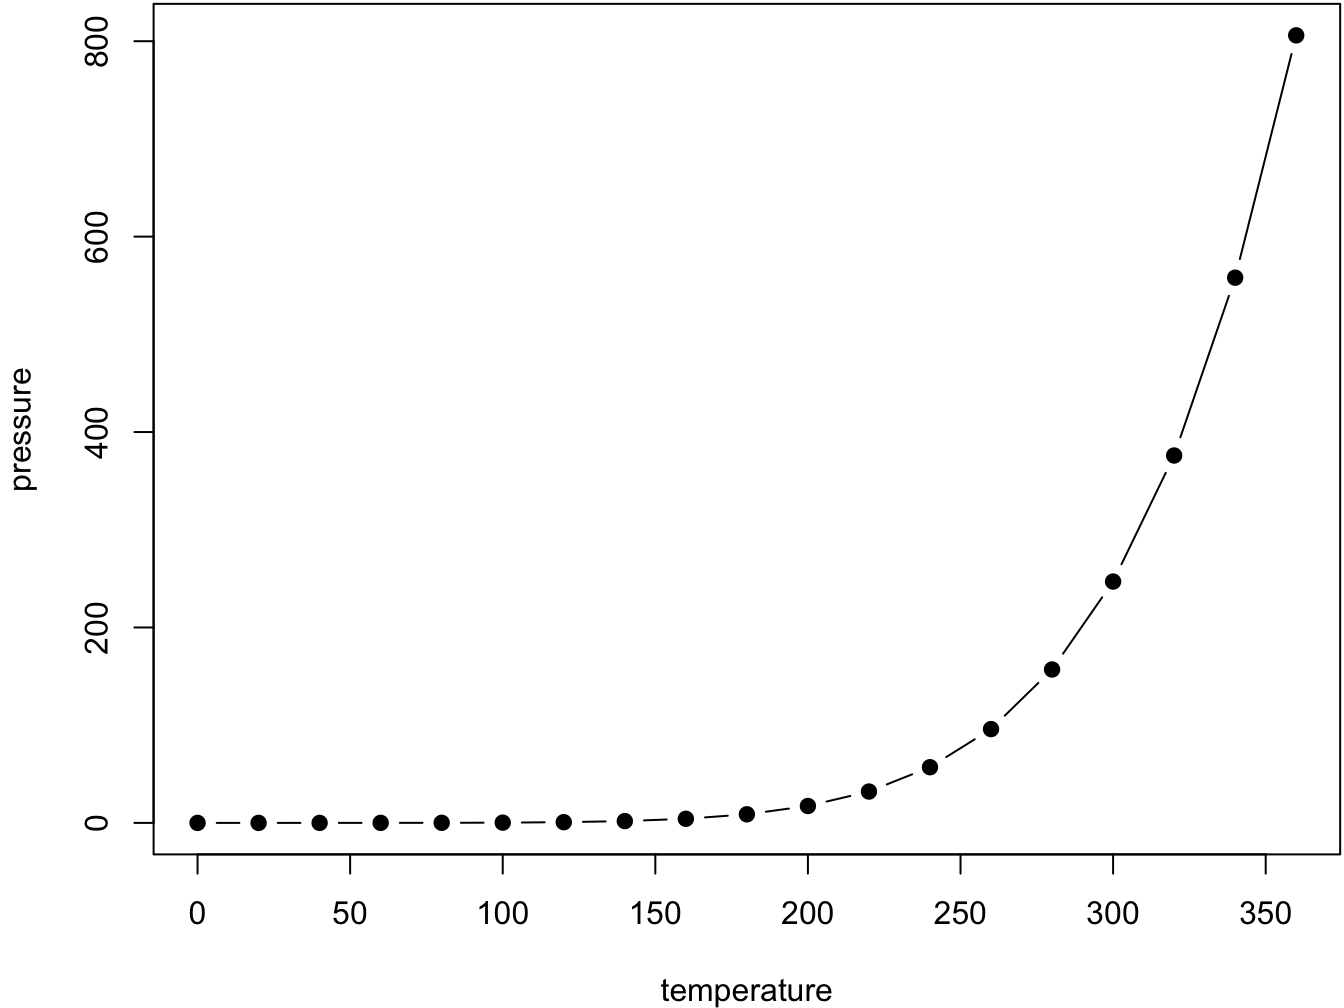
\includegraphics[width=0.8\linewidth]{Field-Trial-Spatial-Analysis-Guide_files/figure-latex/nice-fig-1} 

}

\caption{Here is a nice figure!}\label{fig:nice-fig}
\end{figure}

Reference a figure by its code chunk label with the \texttt{fig:} prefix, e.g., see Figure \ref{fig:nice-fig}. Similarly, you can reference tables generated from \texttt{knitr::kable()}, e.g., see Table \ref{tab:nice-tab}.

\begin{Shaded}
\begin{Highlighting}[]
\NormalTok{knitr}\OperatorTok{::}\KeywordTok{kable}\NormalTok{(}
  \KeywordTok{head}\NormalTok{(iris, }\DecValTok{20}\NormalTok{), }\DataTypeTok{caption =} \StringTok{'Here is a nice table!'}\NormalTok{,}
  \DataTypeTok{booktabs =} \OtherTok{TRUE}
\NormalTok{)}
\end{Highlighting}
\end{Shaded}

\begin{table}[t]

\caption{\label{tab:nice-tab}Here is a nice table!}
\centering
\begin{tabular}{rrrrl}
\toprule
Sepal.Length & Sepal.Width & Petal.Length & Petal.Width & Species\\
\midrule
5.1 & 3.5 & 1.4 & 0.2 & setosa\\
4.9 & 3.0 & 1.4 & 0.2 & setosa\\
4.7 & 3.2 & 1.3 & 0.2 & setosa\\
4.6 & 3.1 & 1.5 & 0.2 & setosa\\
5.0 & 3.6 & 1.4 & 0.2 & setosa\\
\addlinespace
5.4 & 3.9 & 1.7 & 0.4 & setosa\\
4.6 & 3.4 & 1.4 & 0.3 & setosa\\
5.0 & 3.4 & 1.5 & 0.2 & setosa\\
4.4 & 2.9 & 1.4 & 0.2 & setosa\\
4.9 & 3.1 & 1.5 & 0.1 & setosa\\
\addlinespace
5.4 & 3.7 & 1.5 & 0.2 & setosa\\
4.8 & 3.4 & 1.6 & 0.2 & setosa\\
4.8 & 3.0 & 1.4 & 0.1 & setosa\\
4.3 & 3.0 & 1.1 & 0.1 & setosa\\
5.8 & 4.0 & 1.2 & 0.2 & setosa\\
\addlinespace
5.7 & 4.4 & 1.5 & 0.4 & setosa\\
5.4 & 3.9 & 1.3 & 0.4 & setosa\\
5.1 & 3.5 & 1.4 & 0.3 & setosa\\
5.7 & 3.8 & 1.7 & 0.3 & setosa\\
5.1 & 3.8 & 1.5 & 0.3 & setosa\\
\bottomrule
\end{tabular}
\end{table}

You can write citations, too. For example, we are using the \textbf{bookdown} package \citep{R-bookdown} in this sample book, which was built on top of R Markdown and \textbf{knitr} \citep{xie2015}.

\hypertarget{spatial-models-ch2-bg}{%
\chapter{Spatial Models \{ch2-bg\}}\label{spatial-models-ch2-bg}}

This section contains some of the background behind why spatial models are used and how they work. Understanding this section is not essential, but it is extremely helpful. This section relies on information introduced in part I, s please make sure you have read that section, especially if you are new to empirical variograms and spatial statistics.

General linear statistical models are commonly modeled as thus:

\[Y_i = \beta_0 + X_i\beta_1 + \epsilon_i\]
\(\beta_1\) is a slope describing the relationship between a continuous variable and the dependent variable, \(Y_i\). If \(X_i\) is a categorical variable, such as a crop variety, then there will be \(p-1\) slopes estimated, where p is the number of unique treatements levels in \(X\).

The error terms, \(\epsilon_i\) are assumed normally distributed with a mean of zero and a variance of \(\sigma^2\) :

\[e_i ~\sim N(0, \sigma^2)\]
The error terms, or residuals, are assumed to be \emph{identically} and \emph{independently} distributed (abbreviated as ``iid''). This implies a constant variance of the error terms and zero covariance between residuals.

If N = 3, the expanded model looks like this:

\[\left[ {\begin{array}{ccc} Y_1\\ Y_2\\ Y_3 \end{array} } \right] = \beta_0 + 
\left[ {\begin{array}{ccc} X_1\\ X_2\\ X_3 \end{array}  } \right] \beta_1 +
\left[ {\begin{array}{ccc} \epsilon_1\\ \epsilon_2\\ \epsilon_3 \end{array}  } \right] \]

\[e_i ~\sim N \Bigg( 0, 
\left[ {\begin{array}{ccc} \sigma^2 & 0 & 0 \\ 0 & \sigma^2 & 0\\ 0 & 0 & \sigma^2\end{array}  } \right] \Bigg) \]

If spatial variation is present, the off-diagonals of the variance-covariance matrix are not zero - hence the error terms are not independently distributed. As a result, hypotheses test and parameter estimates from uncorrected linear models will provide erroneous results.

\hypertarget{correlated-error-models}{%
\section{Correlated Error Models}\label{correlated-error-models}}

\hypertarget{distance-based-correlation-error-models}{%
\subsection{Distance-based Correlation Error Models}\label{distance-based-correlation-error-models}}

There are mathematical tools for modelling how error terms are correlated with each other based on pairwise physical distance between observations. These models can be used to weight observations. Often, the data are assumed to be \emph{isotropic}, where distance but not direction impacts error spatial correlation

There are several methods for estimating the semivariance as a direct function of distance.

\hypertarget{exponential-model}{%
\subsubsection{Exponential Model}\label{exponential-model}}

\[ \gamma (h)\left\{ {\begin{array}{cc} 0 & h = 0\\ C_0+C_1 \left [ 1-e^{-(\frac{h}{r})} \right] & h > 0 \end{array} } \right. \]
where

\[ C_0 = nugget \\ C_1 = partial \: sill \\ r = range\]

\begin{figure}

{\centering 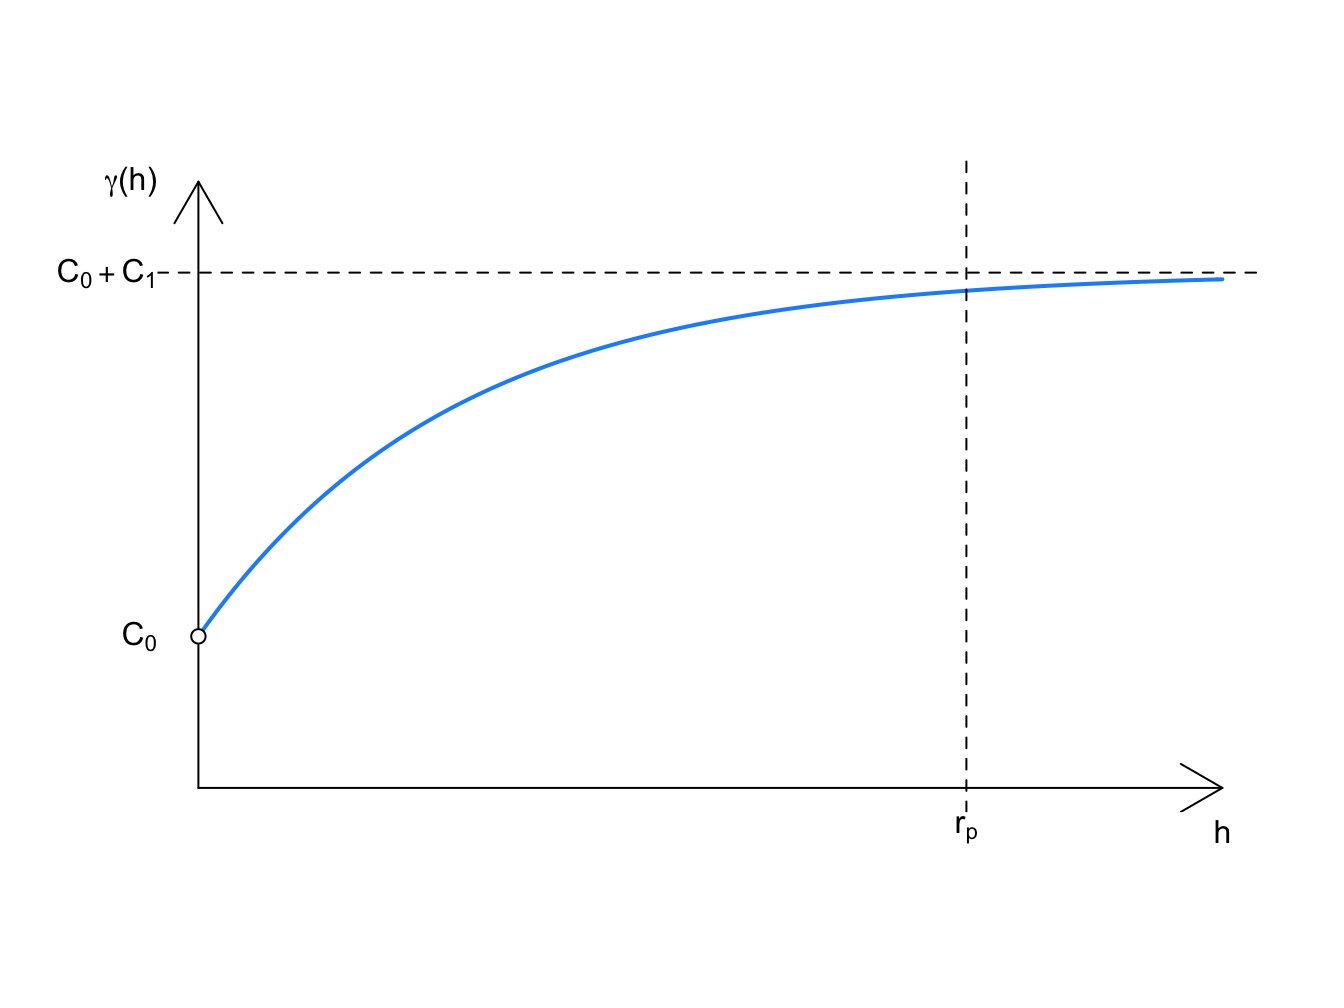
\includegraphics[width=0.7\linewidth]{Field-Trial-Spatial-Analysis-Guide_files/figure-latex/Exp-CE-fig-1} 

}

\caption{Exponential Model}\label{fig:Exp-CE-fig}
\end{figure}

\(3r = r_p\) is the ``practical range'', which is 95\% of the true value for \(C_1\).

\hypertarget{gaussian}{%
\subsubsection{Gaussian}\label{gaussian}}

(a squared version of the exponential model)

\[ \gamma (h)\left\{ {\begin{array}{cc} 0 & h = 0\\ C_0+C_1 \left [ 1-e^{-(\frac{h}{r})^2} \right] & h > 0 \end{array} } \right. \]
where

\[ C_0 = nugget \\ C_1 = partial \: sill \\ r = range\]

\begin{figure}

{\centering 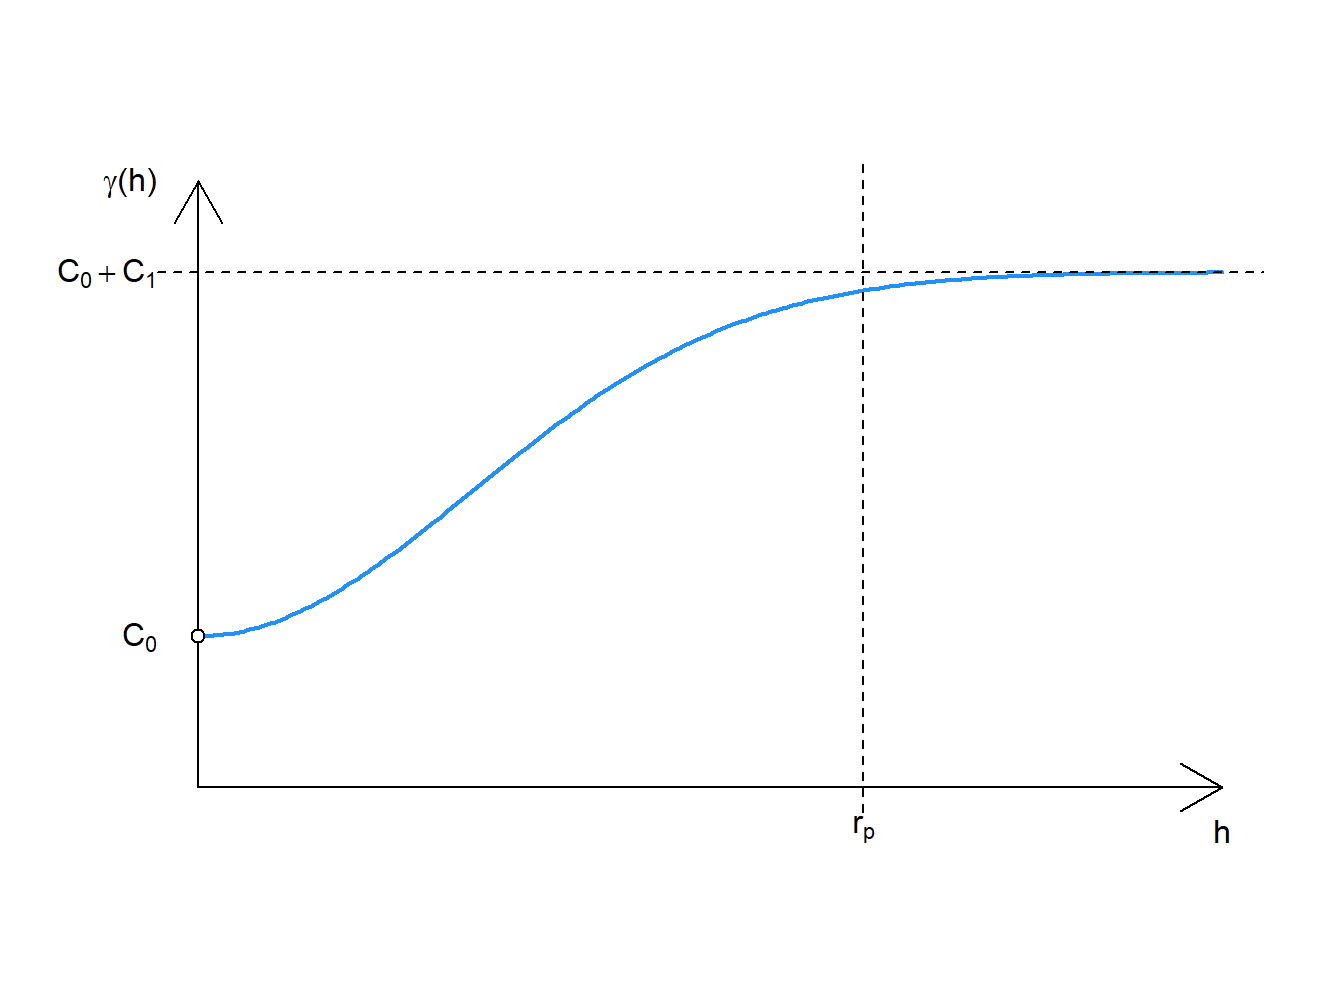
\includegraphics[width=0.7\linewidth]{Field-Trial-Spatial-Analysis-Guide_files/figure-latex/Gau-CE-fig-1} 

}

\caption{Gaussian Model}\label{fig:Gau-CE-fig}
\end{figure}

\(\sqrt 3r = r_p\) is the ``practical range'', which is 95\% of the true value for \(C_1\).

\hypertarget{spherical-model}{%
\subsubsection{Spherical model}\label{spherical-model}}

\[ \gamma (h) = \left\{ {\begin{array}{cc} 0 & h = 0\\ C_0+C_1 \left[ \frac{3h}{2r}-0.5\bigg( \frac{h}{r}\bigg)^3 \right] & 0 <h \leq r \\ 
C_0 + C_1 & h > r \end{array} } \right. \]
where

\[ C_0 = nugget \\ C_1 = partial \: sill \\ r = range\]

\begin{figure}

{\centering 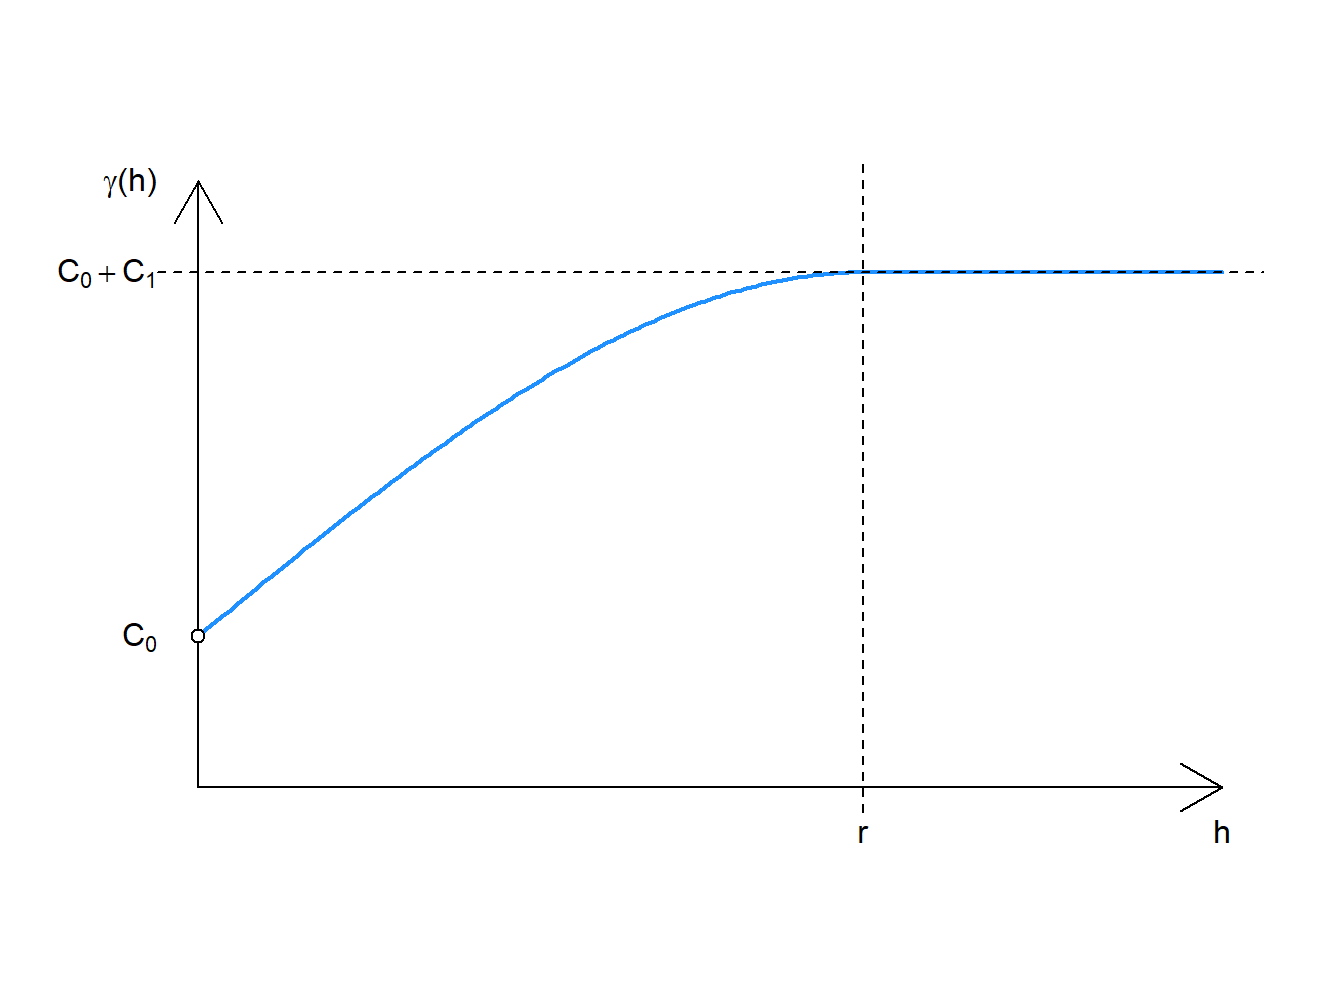
\includegraphics[width=0.7\linewidth]{Field-Trial-Spatial-Analysis-Guide_files/figure-latex/Sph-CE-fig-1} 

}

\caption{Spherical Model}\label{fig:Sph-CE-fig}
\end{figure}

\hypertarget{other-correlated-error-distance-models}{%
\subsubsection{Other correlated error distance models}\label{other-correlated-error-distance-models}}

There are many more models - Matérn, Cauchy, Logistic - that may describe spatial correlation in a data set.

There are two addition models that have no range or sill, the linear model and power model. If your data fits these, consider doing a trend analysis.

\hypertarget{linear-model}{%
\subsubsection{Linear model}\label{linear-model}}

\[ \gamma (h)=\left\{ {\begin{array}{cc} 0 & h = 0\\ C_0+C_1h & h > 0 \end{array} } \right. \]
where

\[ C_0 = nugget \\ C_1 = slope \]

\begin{figure}

{\centering 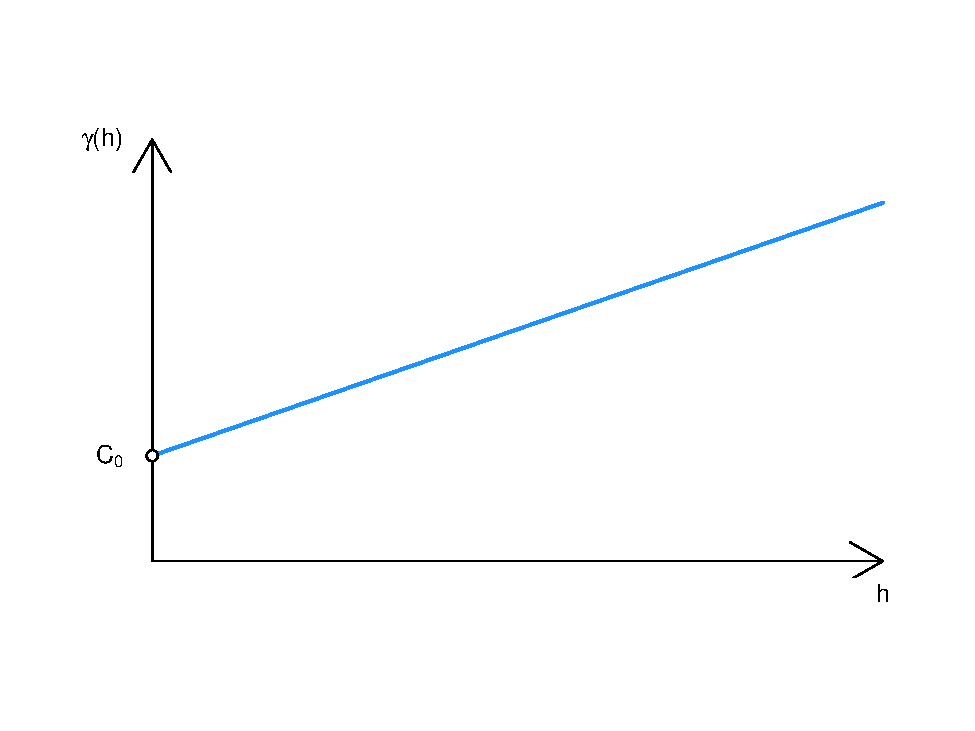
\includegraphics[width=0.7\linewidth]{Field-Trial-Spatial-Analysis-Guide_files/figure-latex/linear-CE-fig-1} 

}

\caption{Linear Error Model}\label{fig:linear-CE-fig}
\end{figure}

There is no sill or range in the linear model, so the variance will continue to increase as a function of distance.

\hypertarget{power-model}{%
\subsubsection{Power Model}\label{power-model}}

\[ \gamma (h)=\left\{ {\begin{array}{cc} 0 & h = 0\\ C_0+C_1h^\lambda & h > 0 \end{array} } \right. \]
where

\[ 0 \leq \lambda <\leq 2 \\ C_0 = nugget \\ C_1 = scaling \: factor \]

\begin{figure}

{\centering 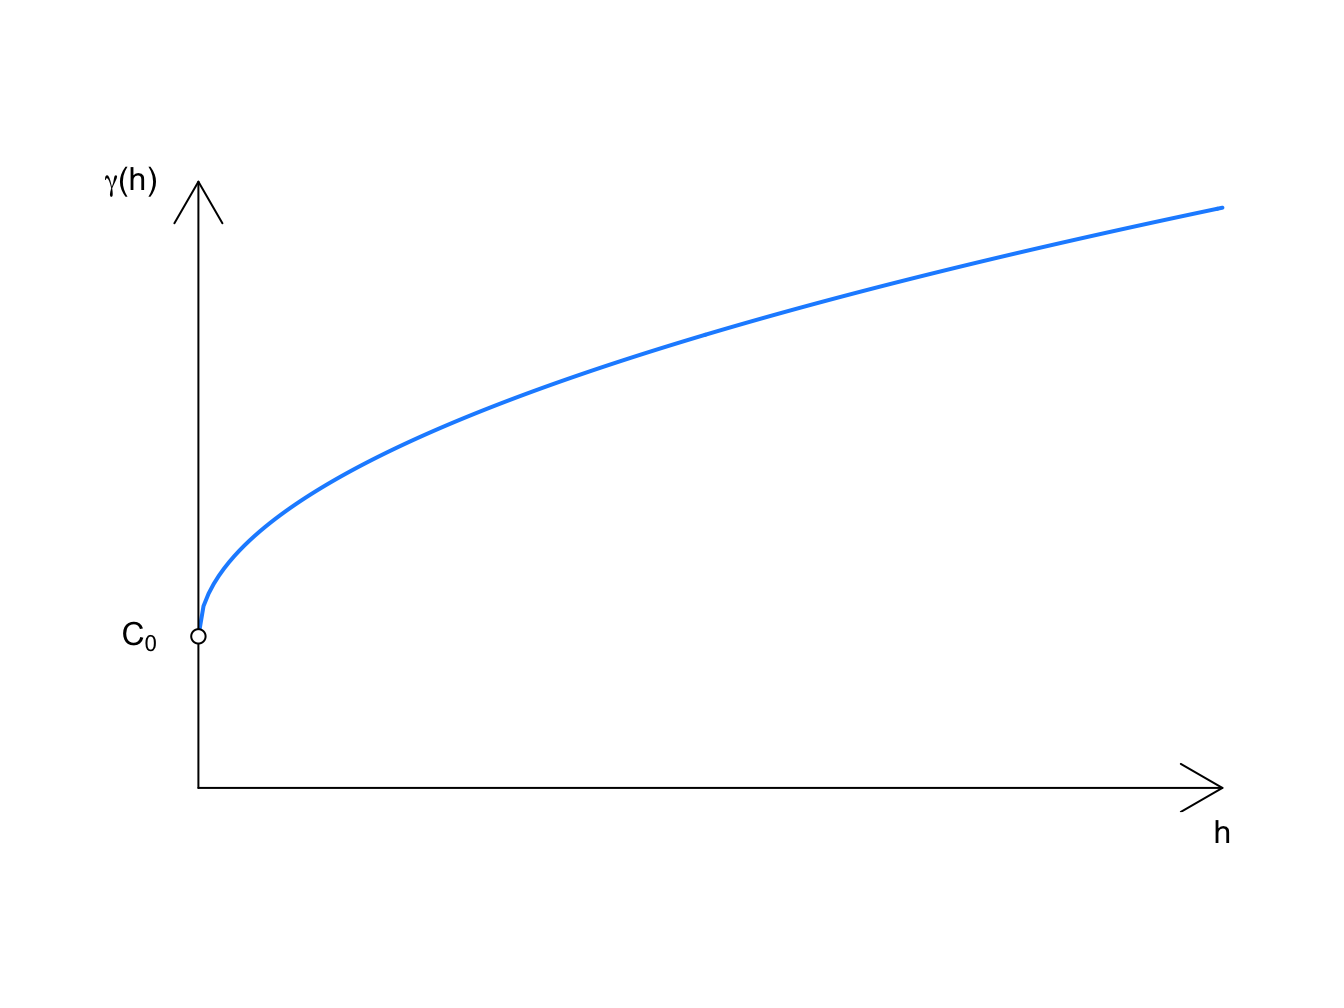
\includegraphics[width=0.7\linewidth]{Field-Trial-Spatial-Analysis-Guide_files/figure-latex/power-CE-fig-1} 

}

\caption{Power Model}\label{fig:power-CE-fig}
\end{figure}

When \(\lambda = 1\), that is equivalent to the linear model. Example above is when \(\lambda = 0.5\) (i.e.~a square-root transformation) and \(C_1 = 1\). There is also no sill or range in the power model.

\hypertarget{correlated-error-models-for-gridded-data}{%
\subsection{Correlated Error Models for Gridded Data}\label{correlated-error-models-for-gridded-data}}

Planned field experiments often have the advantage of being arranged in regular grid pattern that can be adequately described using Euclidian space. This simplifies aspects of understanding how error terms are related by distance since the data occur in evenly spaced increments. Furthermore, in many agricultural trials, there may be no interest in spatial interpolation between units. Some of these models work with irregular data, but the models presented are simplified forms when experimental units are arranged in regular grid.

For example, imagine an experiment consisting of 8 plots (plot = the experiment units) arranged in 2 rows, each with 4 ranges with this layout:

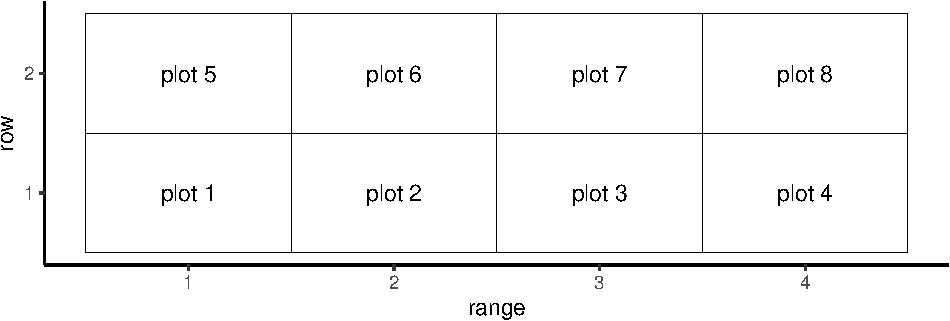
\includegraphics{Field-Trial-Spatial-Analysis-Guide_files/figure-latex/plot-grid-fig-1.pdf}

The statistical model for that experiment:

\[ 
\left[ {\begin{array} \ Y_1 \\ Y_2 \\ \vdots \\ Y_n \end{array} } \right] = \beta_0 + 
\left[ {\begin{array} \ X_1 \\ X_2 \\ \vdots \\ X_n \end{array} } \right] \beta_1 +
\left[ {\begin{array} \ \epsilon_1 \\ \epsilon_2 \\ \vdots \\ \epsilon_n \end{array} } \right]
\]
\(X\beta\) refer to independent variable effects. This same model is also often presented in an abbreviated matrix form:

\[ \mathbf{Y = X\beta + \epsilon}\]

\hypertarget{auto-regressive-model-ar1}{%
\subsubsection{Auto-regressive Model (AR1)}\label{auto-regressive-model-ar1}}

This assumes that variance can be modelled as exponential function based on unit distance (e.g.~row or range), either in a single direction or anistropic.

The AR1 structure across 2 rows is modeled as thus:

\[\mathbf { V_{AR(1)row}}  = \sigma^2
\left[ {\begin{array}{cc} 
1 & \rho \\
\rho & 1 
\end{array} } \right] \otimes \mathbf{I_4} \]

This covariance model describes the correlation of observations in the \emph{row direction only.}

And similarily the AR1 structure across 4 ranges is modeled as thus:

\[ \mathbf {V_{AR(1)range}} = \sigma^2 \mathbf{I_4} \otimes
\left[ {\begin{array}{cccc} 
1 & \rho & \rho^2 & \rho^3 \\
\rho & 1 & \rho & \rho^2  \\
\rho^2 & \rho & 1 & \rho  \\
\rho^3 & \rho^2 & \rho & 1
\end{array} } \right] \]

This covariance model describes the correlation of observations in the \emph{range direction only.}

In combined AR1xAR1 model, the parameter, \(\rho\) may need to estimated separated across the row and column directions depending on the shape of the plots and site-specific field variation. Very rectangular plots are likely to require a separate estimate of the \(\rho\) parameter for each direction.

\$\$ \mathbf {V_{AR(1)row} \otimes V_{AR(1)range}} = \sigma\^{}2
\left[ {\begin{array}{cccc | cccc} 

1 & \rho_1 & \rho_1^2 & \rho_1^3 & \rho_2 & \rho_1\rho_2 & \rho_1^2\rho_2 & \rho_1^3\rho_2 \\
\rho_1 & 1 & \rho_1 & \rho_1^2 & \rho_1\rho_2 & \rho_2 & \rho_1\rho_2 & \rho_1^2\rho_2\\
\rho_1^2 & \rho_1 & 1 & \rho_1 & \rho_1^2\rho_2 & \rho_1\rho_2 & \rho_2 & \rho_1\rho_2\\
\rho_1^3 & \rho_1^2 & \rho_1 & 1 & \rho_1^3\rho_2 & \rho_1^2\rho_2 & \rho_1\rho_2 & \rho_2 \\
\hline
\rho_2 & \rho_1\rho_2 & \rho_1^2\rho_2 & \rho_1^3\rho_2 & 1 & \rho_1 & \rho_1^2 & \rho_1^3 \\
\rho_1\rho_2 & \rho_2 & \rho_1\rho_2 & \rho_1^2\rho_2 & \rho_1 & 1 & \rho_1 & \rho_1^2 \\
\rho_1^2\rho_2 & \rho_1\rho_2 & \rho_2 & \rho_1\rho_2 & \rho_1^2 & \rho_1 & 1 & \rho_1 \\
\rho_1^3\rho_2 & \rho_1^2\rho_2 & \rho_1\rho_2 & \rho_2 &\rho_1^3 & \rho_1^2 & \rho_1 & 1 \\

\end{array} } \right]\$\$

\textbf{Note}: \(\rho_1\) and \(\rho_2\) are the parameter estimate for \(V_{AR1(1) row}\) and \(V_{AR(1)range}\), respectively.

Please note that these error models are for modelling localised variation based on physical proximity. It is assumed that eventually a distance in the experiment can be reached in which 2 observations can be treated independent.
If there are spatial trends that extend along the entire scope of an experiment (for instance, due to position on a slope), then an additional trend analysis should be conducted.

\hypertarget{nearest-neighbor-approaches}{%
\section{Nearest Neighbor Approaches}\label{nearest-neighbor-approaches}}

These approaches look use information from adjacent plots to adjust for spatial auto-correlation.

\hypertarget{spatial-durbin-approach}{%
\subsection{Spatial Durbin Approach}\label{spatial-durbin-approach}}

This one add the average of values the neighboring independent variables to the model:

\[y = X\beta + WX\theta + \epsilon \]

\hypertarget{spatial-autoregressive-sar}{%
\subsection{Spatial Autoregressive (SAR)}\label{spatial-autoregressive-sar}}

Sometimes called a ``lag'' model, the SAR model uses correlations with neighboring plots dependent variable to predict Y. The auto-regressive model explicitly models correlations between neighboring points.

\[\mathbf{Y =  \rho W Y + X\beta + \epsilon} \]

While this may look strange, \(\mathbf{W}\) is an \(n\) x \(n\) matrix weighting the neighbors with a diagonal of zero so the value at \(i=j\), that is \(Y_{ijk}\) itself, is not used on the right-hand side to predict \(Y_{ijk}\) on the left-hand side of the equation. The error terms are assumed iid.

\hypertarget{spatial-error-model-sem}{%
\subsection{Spatial Error Model (SEM)}\label{spatial-error-model-sem}}

This is also refereed to as the ``moving average model'' and is quite similar to auto-regressive model. Auto-regressive models a variables's spatial dependence on nearby experimental units.

\[\mathbf {Y= X\beta + u} \\ \mathbf {u = \lambda W + \nu}\]

Where \(\mathbf{u}\) incorporates both the normally-distributed iid error and spatially correlated error. Like in SAR, \(\mathbf{W}\) is a matrix of spatial weights and \(\lambda\) is a parameter describing autocorrelation of the error terms.

\hypertarget{arima}{%
\subsection{ARIMA}\label{arima}}

The AR1 and MA1 models can be combine into one:

\[ y = X\beta + \rho W_1y+u \\ u = \lambda W_2 + \nu \]

\textbf{On Weights}

Setting weights of neighbors is dealt with in the next chapter\ref{ch3},

\hypertarget{trend-analysis}{%
\section{Trend Analysis}\label{trend-analysis}}

\hypertarget{row-column-and-combined-and-row-plus-column-trends.}{%
\subsection{Row, column and combined and row plus column trends.}\label{row-column-and-combined-and-row-plus-column-trends.}}

Experiment wide-trends should be modeled with directional trend models. These are comparatively simple models:

\[Y_{ijk} = \beta_0 + X_{i1}\beta_1 +  Row_{j2}\beta_2 + Range_{k3}\beta_3 +\epsilon_{ijk}\]

If the assumption of independent, normal, and identical errors are met, then this model will suffice. If spatial variation is still present, additional measures will need to be taken.

\hypertarget{splines}{%
\subsection{Splines}\label{splines}}

There is a rich field of research on using localised splines to model field heterogeneity. These models are complex and hence not described. More resources can be found in the references section.

\hypertarget{ch3}{%
\chapter{Example Analysis}\label{ch3}}

\hypertarget{load-data}{%
\section{Load Data}\label{load-data}}

This tutorial uses the Nebraska Interstate wheat trials, first published by Stroup et al in 1991 and reused extensively in field spatial variation studies.

\begin{Shaded}
\begin{Highlighting}[]
\KeywordTok{library}\NormalTok{(agridat); }\KeywordTok{library}\NormalTok{(dplyr); }\KeywordTok{library}\NormalTok{(tidyr)}
\KeywordTok{data}\NormalTok{(}\StringTok{"stroup.nin"}\NormalTok{)}

\NormalTok{Nin <-}\StringTok{ }\NormalTok{stroup.nin }\OperatorTok\StringTok{ }\KeywordTok{mutate}\NormalTok{(}\DataTypeTok{col.width =}\NormalTok{ col }\OperatorTok{*}\StringTok{ }\FloatTok{1.2}\NormalTok{, }\DataTypeTok{row.length =}\NormalTok{ row }\OperatorTok{*}\StringTok{ }\FloatTok{4.3}\NormalTok{) }\OperatorTok\StringTok{ }
\StringTok{  }\KeywordTok{mutate}\NormalTok{(}\DataTypeTok{name =} \KeywordTok{case_when}\NormalTok{(}\KeywordTok{is.na}\NormalTok{(}\KeywordTok{as.character}\NormalTok{(rep)) }\OperatorTok{~}\StringTok{ }\OtherTok{NA_character_}\NormalTok{, }
                          \OtherTok{TRUE} \OperatorTok{~}\StringTok{ }\KeywordTok{as.character}\NormalTok{(gen))) }\OperatorTok\StringTok{ }\KeywordTok{arrange}\NormalTok{(col, row) }\OperatorTok\StringTok{ }
\StringTok{  }\KeywordTok{mutate}\NormalTok{(}\DataTypeTok{plot =} \DecValTok{1}\OperatorTok{:}\KeywordTok{n}\NormalTok{())}

\NormalTok{Nin.na <-}\StringTok{ }\KeywordTok{filter}\NormalTok{(Nin, }\OperatorTok{!}\KeywordTok{is.na}\NormalTok{(rep))}
\end{Highlighting}
\end{Shaded}

\hypertarget{examine-data}{%
\subsection{Examine Data}\label{examine-data}}

\begin{Shaded}
\begin{Highlighting}[]
\KeywordTok{head}\NormalTok{(Nin)}
\end{Highlighting}
\end{Shaded}

\begin{verbatim}
##        gen  rep yield col row col.width row.length     name plot
## 1   Lancer <NA>    NA   1   1       1.2        4.3     <NA>    1
## 2  NE83407   R1 19.40   1   2       1.2        8.6  NE83407    2
## 3 Buckskin   R1 29.85   1   3       1.2       12.9 Buckskin    3
## 4  NE87612   R1 28.15   1   4       1.2       17.2  NE87612    4
## 5     Vona   R2 26.80   1   5       1.2       21.5     Vona    5
## 6  NE87512   R2 20.20   1   6       1.2       25.8  NE87512    6
\end{verbatim}

\begin{Shaded}
\begin{Highlighting}[]
\KeywordTok{str}\NormalTok{(Nin)}
\end{Highlighting}
\end{Shaded}

\begin{verbatim}
## 'data.frame':    242 obs. of  9 variables:
##  $ gen       : Factor w/ 56 levels "Arapahoe","Brule",..: 12 16 3 44 56 41 34 7 3 44 ...
##  $ rep       : Factor w/ 4 levels "R1","R2","R3",..: NA 1 1 1 2 2 3 3 3 4 ...
##  $ yield     : num  NA 19.4 29.9 28.1 26.8 ...
##  $ col       : int  1 1 1 1 1 1 1 1 1 1 ...
##  $ row       : int  1 2 3 4 5 6 7 8 9 10 ...
##  $ col.width : num  1.2 1.2 1.2 1.2 1.2 1.2 1.2 1.2 1.2 1.2 ...
##  $ row.length: num  4.3 8.6 12.9 17.2 21.5 25.8 30.1 34.4 38.7 43 ...
##  $ name      : chr  NA "NE83407" "Buckskin" "NE87612" ...
##  $ plot      : int  1 2 3 4 5 6 7 8 9 10 ...
\end{verbatim}

This data set actually has no missing data -- this is a balanced trial. However, there are empty fill plot with no data which creates some issues regarding NA handling.

Plot raw data as it appeared in the field:

\begin{Shaded}
\begin{Highlighting}[]
\KeywordTok{library}\NormalTok{(ggplot2); }\KeywordTok{library}\NormalTok{(desplot)}
\end{Highlighting}
\end{Shaded}

\begin{Shaded}
\begin{Highlighting}[]
\KeywordTok{ggplot}\NormalTok{(Nin, }\KeywordTok{aes}\NormalTok{(}\DataTypeTok{x =}\NormalTok{ row, }\DataTypeTok{y =}\NormalTok{ col)) }\OperatorTok{+}
\StringTok{  }\KeywordTok{geom_tile}\NormalTok{(}\KeywordTok{aes}\NormalTok{(}\DataTypeTok{fill =}\NormalTok{ yield), }\DataTypeTok{col =} \StringTok{"white"}\NormalTok{) }\OperatorTok{+}
\StringTok{  }\CommentTok{#geom_text(aes(label = name)) +}
\StringTok{  }\KeywordTok{geom_text}\NormalTok{(}\KeywordTok{aes}\NormalTok{(}\DataTypeTok{label =}\NormalTok{ plot)) }\OperatorTok{+}
\StringTok{  }\KeywordTok{geom_tileborder}\NormalTok{(}\KeywordTok{aes}\NormalTok{(}\DataTypeTok{group =} \DecValTok{1}\NormalTok{, }\DataTypeTok{grp =}\NormalTok{ rep), }\DataTypeTok{lwd =} \FloatTok{1.2}\NormalTok{) }\OperatorTok{+}
\StringTok{  }\KeywordTok{scale_fill_gradient}\NormalTok{(}\DataTypeTok{low =} \StringTok{"white"}\NormalTok{, }\DataTypeTok{high =} \StringTok{"blue"}\NormalTok{) }\OperatorTok{+}
\StringTok{  }\KeywordTok{scale_x_continuous}\NormalTok{(}\DataTypeTok{breaks =} \KeywordTok{seq}\NormalTok{(}\DecValTok{1}\NormalTok{,}\KeywordTok{max}\NormalTok{(Nin}\OperatorTok{$}\NormalTok{row), }\DecValTok{1}\NormalTok{)) }\OperatorTok{+}
\StringTok{  }\KeywordTok{scale_y_continuous}\NormalTok{(}\DataTypeTok{breaks =} \DecValTok{1}\OperatorTok{:}\KeywordTok{max}\NormalTok{(Nin}\OperatorTok{$}\NormalTok{col)) }\OperatorTok{+}
\StringTok{  }\KeywordTok{labs}\NormalTok{(}\DataTypeTok{x =} \StringTok{"row"}\NormalTok{, }\DataTypeTok{y =} \StringTok{"column"}\NormalTok{, }\DataTypeTok{title =} \StringTok{"field plot layout"}\NormalTok{) }\OperatorTok{+}\StringTok{ }
\StringTok{  }\KeywordTok{theme_classic}\NormalTok{() }\OperatorTok{+}
\StringTok{  }\KeywordTok{theme}\NormalTok{(}\DataTypeTok{axis.text =} \KeywordTok{element_text}\NormalTok{(}\DataTypeTok{size =} \DecValTok{12}\NormalTok{),}
        \DataTypeTok{axis.title =} \KeywordTok{element_text}\NormalTok{(}\DataTypeTok{size =} \DecValTok{14}\NormalTok{),}
        \DataTypeTok{legend.title =} \KeywordTok{element_text}\NormalTok{(}\DataTypeTok{size =} \DecValTok{14}\NormalTok{),}
        \DataTypeTok{legend.text =} \KeywordTok{element_text}\NormalTok{(}\DataTypeTok{size =} \DecValTok{12}\NormalTok{))}
\end{Highlighting}
\end{Shaded}

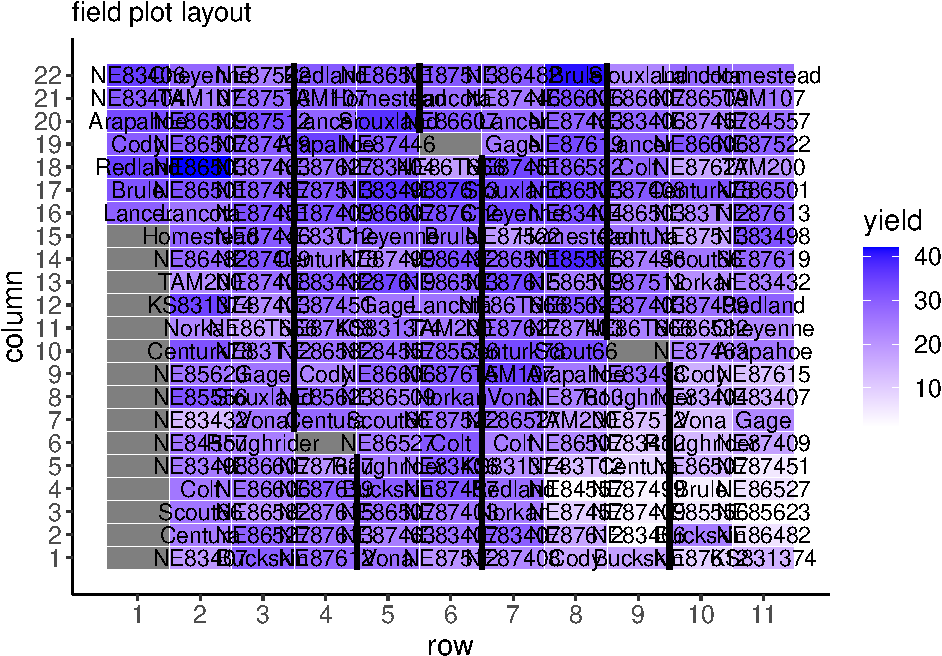
\includegraphics{Field-Trial-Spatial-Analysis-Guide_files/figure-latex/Nin-yield-layout-fig-1.pdf}
Black lines delineate the blocks.

\begin{Shaded}
\begin{Highlighting}[]
\KeywordTok{library}\NormalTok{(rayshader)}
\KeywordTok{options}\NormalTok{(}\DataTypeTok{cores =} \DecValTok{3}\NormalTok{)}
\end{Highlighting}
\end{Shaded}

It's also helpful to plot raw response data:

\begin{Shaded}
\begin{Highlighting}[]
\KeywordTok{par}\NormalTok{(}\DataTypeTok{mfrow=}\KeywordTok{c}\NormalTok{(}\DecValTok{1}\NormalTok{,}\DecValTok{3}\NormalTok{))}
\KeywordTok{boxplot}\NormalTok{(yield }\OperatorTok{~}\StringTok{ }\NormalTok{rep, }\DataTypeTok{data =}\NormalTok{ Nin, }\DataTypeTok{xlab =} \StringTok{"rep"}\NormalTok{, }\DataTypeTok{ylab =} \StringTok{"yield (bu/acres)"}\NormalTok{, }\DataTypeTok{col =} \StringTok{"red2"}\NormalTok{, }\DataTypeTok{main =} \StringTok{"yield across blocks"}\NormalTok{)}
\KeywordTok{boxplot}\NormalTok{(yield }\OperatorTok{~}\StringTok{ }\NormalTok{row, }\DataTypeTok{data =}\NormalTok{ Nin, }\DataTypeTok{xlab =} \StringTok{"row"}\NormalTok{, }\DataTypeTok{ylab =} \StringTok{"yield (bu/acres)"}\NormalTok{,}\DataTypeTok{col =} \StringTok{"dodgerblue2"}\NormalTok{, }\DataTypeTok{main =} \StringTok{"yield across rows"}\NormalTok{)}
\KeywordTok{boxplot}\NormalTok{(yield }\OperatorTok{~}\StringTok{ }\NormalTok{col, }\DataTypeTok{data =}\NormalTok{ Nin, }\DataTypeTok{col =} \StringTok{"gold"}\NormalTok{, }\DataTypeTok{xlab =} \StringTok{"column"}\NormalTok{, }\DataTypeTok{ylab =} \StringTok{"yield (bu/acres)"}\NormalTok{,}\DataTypeTok{main =} \StringTok{"yield across columns"}\NormalTok{)}
\end{Highlighting}
\end{Shaded}

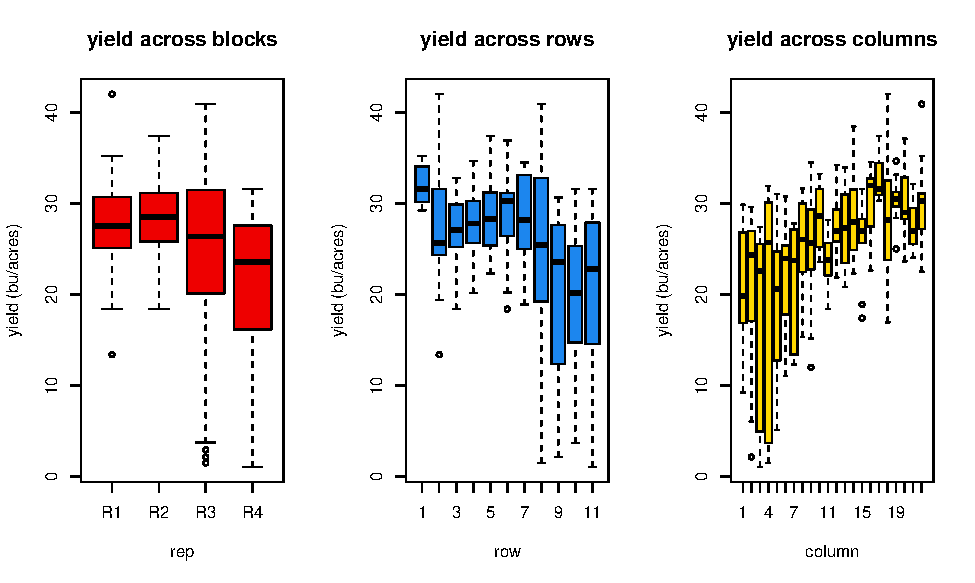
\includegraphics{Field-Trial-Spatial-Analysis-Guide_files/figure-latex/Nin-boxplot-fig-1.pdf}

\begin{Shaded}
\begin{Highlighting}[]
\KeywordTok{par}\NormalTok{(}\DataTypeTok{mfrow=}\KeywordTok{c}\NormalTok{(}\DecValTok{1}\NormalTok{,}\DecValTok{1}\NormalTok{))}
\end{Highlighting}
\end{Shaded}

\hypertarget{test-for-spatial-correlation}{%
\section{Test for Spatial Correlation}\label{test-for-spatial-correlation}}

\hypertarget{morans-i-1}{%
\subsection{Moran's I}\label{morans-i-1}}

First, run a standard linear model of the experiment:

\begin{Shaded}
\begin{Highlighting}[]
\KeywordTok{library}\NormalTok{(nlme); }\KeywordTok{library}\NormalTok{(car)}

\NormalTok{nin.lme <-}\StringTok{ }\KeywordTok{lme}\NormalTok{(yield }\OperatorTok{~}\StringTok{ }\NormalTok{gen, }\DataTypeTok{random =} \OperatorTok{~}\DecValTok{1}\OperatorTok{|}\NormalTok{rep,}
              \DataTypeTok{data =}\NormalTok{ Nin,}
              \DataTypeTok{na.action =}\NormalTok{ na.exclude)}

\KeywordTok{Anova}\NormalTok{(nin.lme, }\DataTypeTok{type =} \StringTok{"2"}\NormalTok{)}
\end{Highlighting}
\end{Shaded}

\begin{verbatim}
## Analysis of Deviance Table (Type II tests)
## 
## Response: yield
##      Chisq Df Pr(>Chisq)
## gen 48.152 55     0.7317
\end{verbatim}

Next, establish and weight neighbors. In this example, only adjacent neighbors in the rook formation are used and are weighted proportionally according to their representation as neighbors to an individual. That is, if a unit has 4 adjacent neighbors, each neighbor is weighted as 0.25. If there are only two neighbors, each is weighted as 0.5.

The function \texttt{cell2nb} is a simplified function for setting neighbors when working with data laid out in a regular grid, which is a common feature of many agricultural field trials.

\begin{Shaded}
\begin{Highlighting}[]
\KeywordTok{library}\NormalTok{(spdep)}
\NormalTok{xy.rook <-}\StringTok{ }\KeywordTok{cell2nb}\NormalTok{(}\DataTypeTok{nrow =} \KeywordTok{max}\NormalTok{(Nin}\OperatorTok{$}\NormalTok{row), }\DataTypeTok{ncol =} \KeywordTok{max}\NormalTok{(Nin}\OperatorTok{$}\NormalTok{col), }\DataTypeTok{type=}\StringTok{"rook"}\NormalTok{) }\CommentTok{# make sur your data sorted by the variables assigned to row and col (in that order), and there is one and only one observation in the data set for each unique row/col combination. Even missing plots need a row}
\end{Highlighting}
\end{Shaded}

\emph{Rook adjacency plot for the NIN data}

\begin{Shaded}
\begin{Highlighting}[]
\KeywordTok{library}\NormalTok{(sf)}
\KeywordTok{plot}\NormalTok{(xy.rook, }\DataTypeTok{coords =} \KeywordTok{st_multipoint}\NormalTok{(}\KeywordTok{matrix}\NormalTok{(}\KeywordTok{c}\NormalTok{(Nin}\OperatorTok{$}\NormalTok{col, Nin}\OperatorTok{$}\NormalTok{row), }\DataTypeTok{ncol =} \DecValTok{2}\NormalTok{)))}
\end{Highlighting}
\end{Shaded}

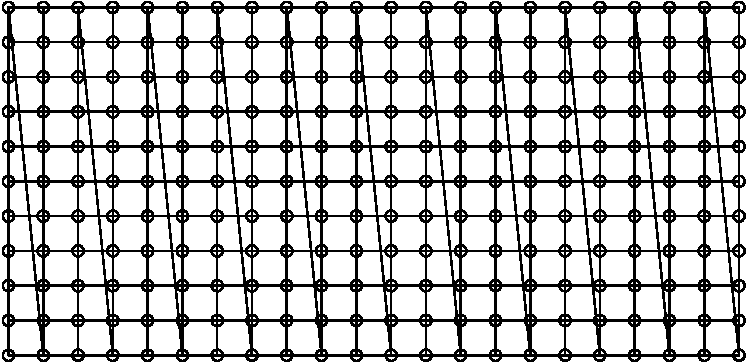
\includegraphics{Field-Trial-Spatial-Analysis-Guide_files/figure-latex/nin-rook-adj-fg-1.pdf}
Each observation considers ``neighbors'' to be those which touch the cell in a row or column oriention, but not diagonal.

Conduct Moran's test via standard t-test and using MC sampling.

\begin{Shaded}
\begin{Highlighting}[]
\NormalTok{resid.lme <-}\StringTok{ }\KeywordTok{residuals}\NormalTok{(nin.lme)}
\KeywordTok{names}\NormalTok{(resid.lme) <-}\StringTok{ }\NormalTok{Nin}\OperatorTok{$}\NormalTok{plot}
\KeywordTok{moran.test}\NormalTok{(resid.lme, }\KeywordTok{nb2listw}\NormalTok{(xy.rook), }\DataTypeTok{na.action =}\NormalTok{ na.exclude)}
\end{Highlighting}
\end{Shaded}

\begin{verbatim}
## 
##  Moran I test under randomisation
## 
## data:  resid.lme  
## weights: nb2listw(xy.rook) 
## omitted: 1, 12, 23, 34, 45, 56, 59, 67, 78, 89, 100, 108, 111, 122, 133, 144, 155, 204   
## 
## Moran I statistic standard deviate = 8.1602, p-value < 2.2e-16
## alternative hypothesis: greater
## sample estimates:
## Moran I statistic       Expectation          Variance 
##       0.402504491      -0.004484305       0.002487522
\end{verbatim}

\begin{Shaded}
\begin{Highlighting}[]
\KeywordTok{moran.mc}\NormalTok{(resid.lme, }\KeywordTok{nb2listw}\NormalTok{(xy.rook), }\DecValTok{999}\NormalTok{, }\DataTypeTok{na.action =}\NormalTok{ na.exclude)}
\end{Highlighting}
\end{Shaded}

\begin{verbatim}
## 
##  Monte-Carlo simulation of Moran I
## 
## data:  resid.lme 
## weights: nb2listw(xy.rook) 
## omitted: 1, 12, 23, 34, 45, 56, 59, 67, 78, 89, 100, 108, 111, 122, 133, 144, 155, 204 
## number of simulations + 1: 1000 
## 
## statistic = 0.4025, observed rank = 1000, p-value = 0.001
## alternative hypothesis: greater
\end{verbatim}

Plot Spatial dependence of resids

\begin{Shaded}
\begin{Highlighting}[]
\KeywordTok{library}\NormalTok{(purrr)}
\NormalTok{res.nn1 <-}\StringTok{ }\KeywordTok{map_dbl}\NormalTok{(xy.rook, }\ControlFlowTok{function}\NormalTok{(j) }\KeywordTok{mean}\NormalTok{(resid.lme[j]))}
  
\NormalTok{c <-}\StringTok{ }\KeywordTok{signif}\NormalTok{(}\KeywordTok{cor}\NormalTok{(resid.lme, res.nn1, }\DataTypeTok{use =} \StringTok{"pairwise.complete.obs"}\NormalTok{), }\DecValTok{2}\NormalTok{)}

\KeywordTok{plot}\NormalTok{(}\DataTypeTok{x =}\NormalTok{ resid.lme, }\DataTypeTok{y =}\NormalTok{ res.nn1, }
     \DataTypeTok{main =} \KeywordTok{paste0}\NormalTok{(}\StringTok{"r = "}\NormalTok{, c), }\DataTypeTok{xlab =} \StringTok{"residual"}\NormalTok{, }\DataTypeTok{ylab =} \StringTok{"average residual of neighbor (rook)"}\NormalTok{)}
\end{Highlighting}
\end{Shaded}

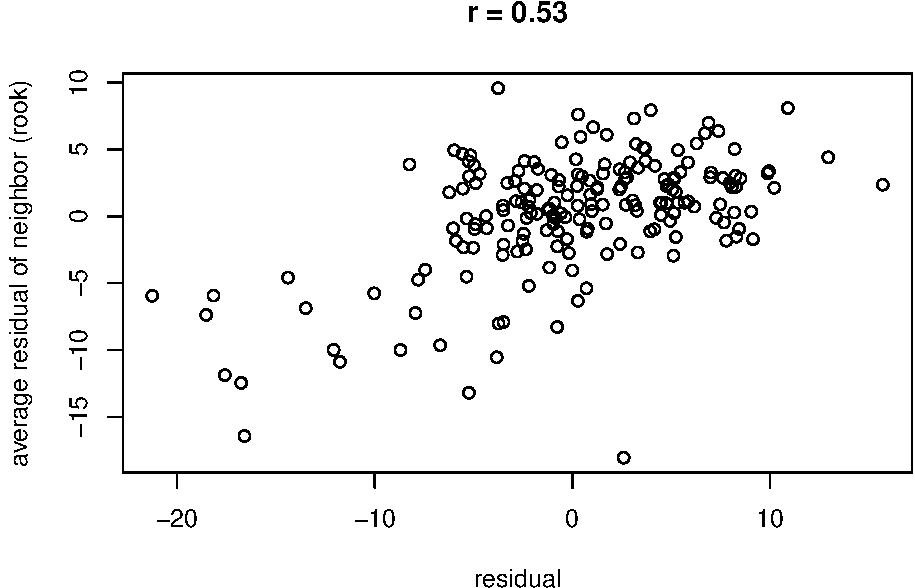
\includegraphics{Field-Trial-Spatial-Analysis-Guide_files/figure-latex/resid-cor-fig-1.pdf}

\hypertarget{note-on-gearys-c}{%
\subsection{Note on Geary's C}\label{note-on-gearys-c}}

At this time, the spdep function \texttt{geary.test()} for Geary's C does not handle missing spatial points. This is area to contribute to! The

\hypertarget{empirical-variogram-fitting}{%
\section{Empirical Variogram Fitting}\label{empirical-variogram-fitting}}

First, create a spatial object by adding spatial coordinates to an ordinary data frame. I like to use the actual units of the plots since they are exaggerated rectangals (meters in this example).

\begin{Shaded}
\begin{Highlighting}[]
\NormalTok{Nin.spatial <-}\StringTok{ }\NormalTok{Nin.na}
\KeywordTok{coordinates}\NormalTok{(Nin.spatial) <-}\StringTok{ }\ErrorTok{~}\StringTok{ }\NormalTok{col.width }\OperatorTok{+}\StringTok{ }\NormalTok{row.length}
\KeywordTok{class}\NormalTok{(Nin.spatial)}
\end{Highlighting}
\end{Shaded}

\begin{verbatim}
## [1] "SpatialPointsDataFrame"
## attr(,"package")
## [1] "sp"
\end{verbatim}

Set the maximum distance for calculating the variogram model (which is one-half the maximum distance between two points).

\begin{Shaded}
\begin{Highlighting}[]
\NormalTok{max_dist =}\StringTok{ }\FloatTok{0.6}\OperatorTok{*}\KeywordTok{max}\NormalTok{(}\KeywordTok{dist}\NormalTok{(}\KeywordTok{coordinates}\NormalTok{(Nin.spatial)))}
\NormalTok{max_dist}
\end{Highlighting}
\end{Shaded}

\begin{verbatim}
## [1] 29.90409
\end{verbatim}

Calculate semivariance for an istropic model and plot the variogram.

\begin{Shaded}
\begin{Highlighting}[]
\KeywordTok{library}\NormalTok{(gstat)}
\NormalTok{resid.var1 <-}\StringTok{ }\KeywordTok{variogram}\NormalTok{(yield }\OperatorTok{~}\StringTok{ }\NormalTok{rep }\OperatorTok{+}\StringTok{ }\NormalTok{gen, }
                        \DataTypeTok{cutoff =}\NormalTok{ max_dist,}
                        \DataTypeTok{width =}\NormalTok{ max_dist}\OperatorTok{/}\DecValTok{20}\NormalTok{, }\CommentTok{# 20 is the number of bins}
                        \DataTypeTok{data =}\NormalTok{ Nin.spatial)}
\KeywordTok{plot}\NormalTok{(resid.var1)}
\end{Highlighting}
\end{Shaded}

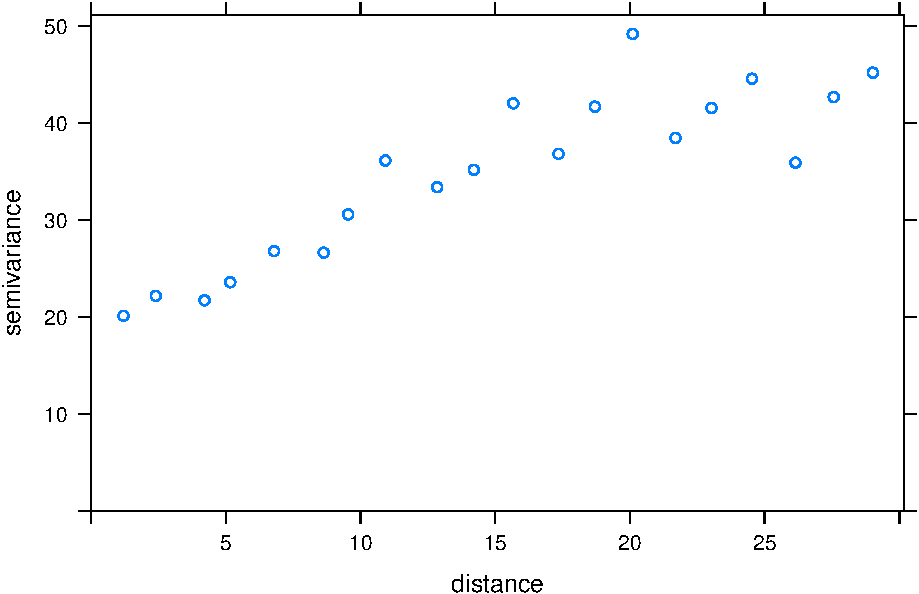
\includegraphics{Field-Trial-Spatial-Analysis-Guide_files/figure-latex/unnamed-chunk-14-1.pdf}

Test out correlated error models:

First, set the starting nugget values as the minimum of the semi-variance. There is likely more sophicated methods to establish the starting value for nugget, but I have found that extracting the minimum value of the semivariance to work well as a starting point.

\begin{Shaded}
\begin{Highlighting}[]
\NormalTok{nugget_start <-}\StringTok{ }\KeywordTok{min}\NormalTok{(resid.var1}\OperatorTok{$}\NormalTok{gamma)}
\end{Highlighting}
\end{Shaded}

Establish models for variogram fitting.

\begin{Shaded}
\begin{Highlighting}[]
\NormalTok{Nin.vgm1 <-}\StringTok{ }\KeywordTok{vgm}\NormalTok{(}\DataTypeTok{model =} \StringTok{"Exp"}\NormalTok{, }\DataTypeTok{nugget =}\NormalTok{ nugget_start) }\CommentTok{# exponential}
\NormalTok{Nin.vgm2 <-}\StringTok{ }\KeywordTok{vgm}\NormalTok{(}\DataTypeTok{model =} \StringTok{"Sph"}\NormalTok{, }\DataTypeTok{nugget =}\NormalTok{ nugget_start) }\CommentTok{# spherical}
\NormalTok{Nin.vgm3 <-}\StringTok{ }\KeywordTok{vgm}\NormalTok{(}\DataTypeTok{model =} \StringTok{"Gau"}\NormalTok{, }\DataTypeTok{nugget =}\NormalTok{ nugget_start) }\CommentTok{# Gaussian}
\end{Highlighting}
\end{Shaded}

Fit the variograms to the data:

\begin{Shaded}
\begin{Highlighting}[]
\NormalTok{Nin.variofit1 <-}\StringTok{ }\KeywordTok{fit.variogram}\NormalTok{(resid.var1, Nin.vgm1)}
\NormalTok{Nin.variofit2 <-}\StringTok{ }\KeywordTok{fit.variogram}\NormalTok{(resid.var1, Nin.vgm2)}
\NormalTok{Nin.variofit3 <-}\StringTok{ }\KeywordTok{fit.variogram}\NormalTok{(resid.var1, Nin.vgm3)}
\end{Highlighting}
\end{Shaded}

Look at the results! (this is fun)

\begin{Shaded}
\begin{Highlighting}[]
\KeywordTok{plot}\NormalTok{(resid.var1, Nin.variofit1, }\DataTypeTok{main =} \StringTok{"Exponential model"}\NormalTok{)}
\end{Highlighting}
\end{Shaded}

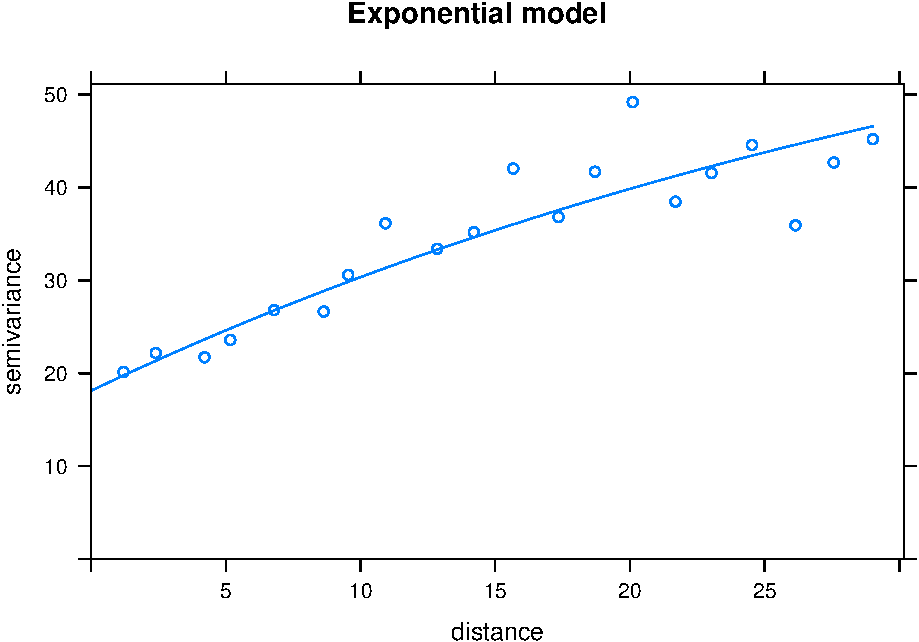
\includegraphics{Field-Trial-Spatial-Analysis-Guide_files/figure-latex/unnamed-chunk-18-1.pdf}

\begin{Shaded}
\begin{Highlighting}[]
\KeywordTok{plot}\NormalTok{(resid.var1, Nin.variofit2, }\DataTypeTok{main =} \StringTok{"Spherical model"}\NormalTok{)}
\end{Highlighting}
\end{Shaded}

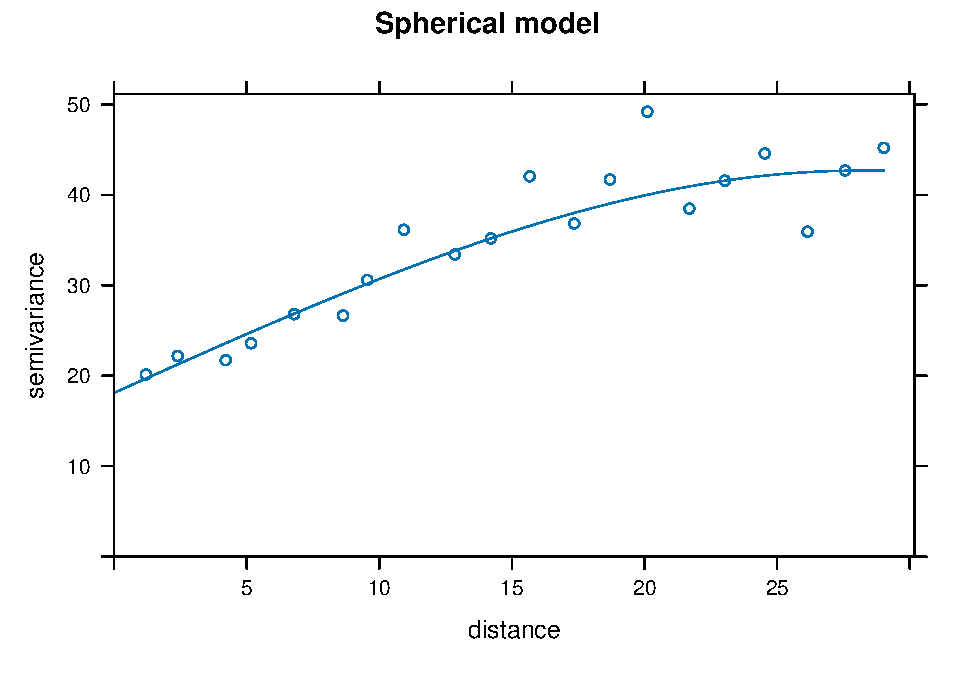
\includegraphics{Field-Trial-Spatial-Analysis-Guide_files/figure-latex/unnamed-chunk-18-2.pdf}

\begin{Shaded}
\begin{Highlighting}[]
\KeywordTok{plot}\NormalTok{(resid.var1, Nin.variofit3, }\DataTypeTok{main =} \StringTok{"Gaussian model"}\NormalTok{)}
\end{Highlighting}
\end{Shaded}

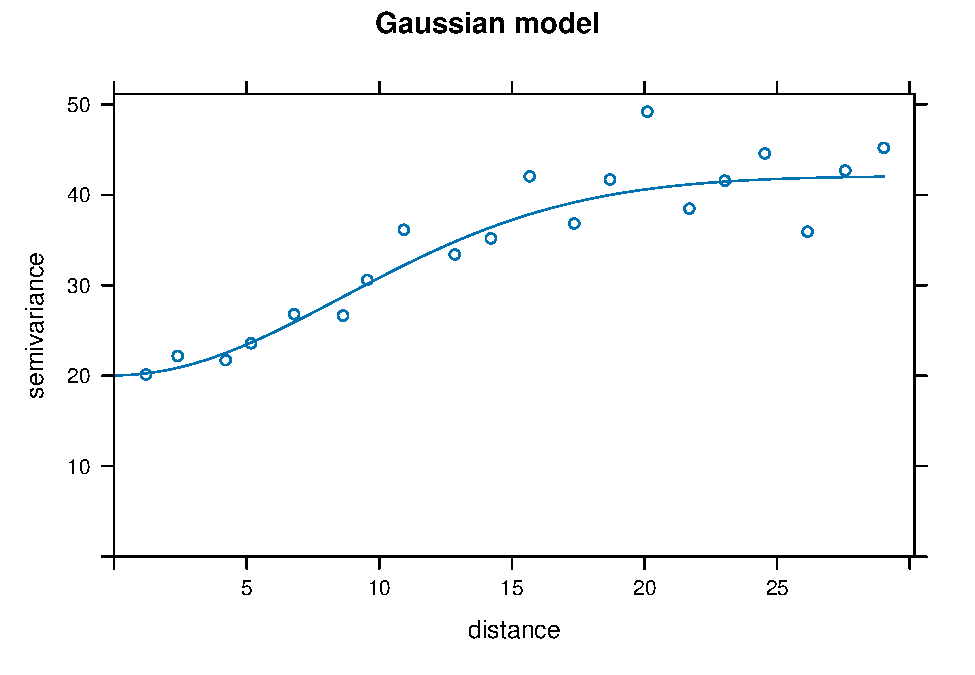
\includegraphics{Field-Trial-Spatial-Analysis-Guide_files/figure-latex/unnamed-chunk-18-3.pdf}

How to pick the best one? Looking at how well each captures the error is the best approach. The attribute ``SSError'' indicates how well each model was able to predict the binned error terms as a function of distance.

\begin{Shaded}
\begin{Highlighting}[]
\KeywordTok{print}\NormalTok{(}\StringTok{"Exponential"}\NormalTok{); }\KeywordTok{attr}\NormalTok{(Nin.variofit1, }\StringTok{"SSErr"}\NormalTok{)}
\end{Highlighting}
\end{Shaded}

\begin{verbatim}
## [1] "Exponential"
\end{verbatim}

\begin{verbatim}
## [1] 1129.799
\end{verbatim}

\begin{Shaded}
\begin{Highlighting}[]
\KeywordTok{print}\NormalTok{(}\StringTok{"Spherical"}\NormalTok{); }\KeywordTok{attr}\NormalTok{(Nin.variofit2, }\StringTok{"SSErr"}\NormalTok{)}
\end{Highlighting}
\end{Shaded}

\begin{verbatim}
## [1] "Spherical"
\end{verbatim}

\begin{verbatim}
## [1] 1012.76
\end{verbatim}

\begin{Shaded}
\begin{Highlighting}[]
\KeywordTok{print}\NormalTok{(}\StringTok{"Gaussian"}\NormalTok{); }\KeywordTok{attr}\NormalTok{(Nin.variofit3, }\StringTok{"SSErr"}\NormalTok{)}
\end{Highlighting}
\end{Shaded}

\begin{verbatim}
## [1] "Gaussian"
\end{verbatim}

\begin{verbatim}
## [1] 752.5491
\end{verbatim}

\texttt{Nin.Variofit3} had the lowest error terms, corresponding to the Gaussian model.

Results from the empirical variogram:

\begin{Shaded}
\begin{Highlighting}[]
\NormalTok{Nin.variofit3}
\end{Highlighting}
\end{Shaded}

\begin{verbatim}
##   model    psill    range
## 1   Nug 20.04106  0.00000
## 2   Gau 22.04013 12.19921
\end{verbatim}

The variogram parameters can be easily extracted from this table:

\begin{Shaded}
\begin{Highlighting}[]
\NormalTok{nugget <-}\StringTok{ }\NormalTok{Nin.variofit3}\OperatorTok{$}\NormalTok{psill[}\DecValTok{1}\NormalTok{] }\CommentTok{# "measurement error"}
\NormalTok{range <-}\StringTok{ }\NormalTok{Nin.variofit3}\OperatorTok{$}\NormalTok{range[}\DecValTok{2}\NormalTok{] }\CommentTok{# distance to establish independence between data points}
\NormalTok{sill <-}\StringTok{ }\KeywordTok{sum}\NormalTok{(Nin.variofit3}\OperatorTok{$}\NormalTok{psill) }\CommentTok{# maximum semivariance}
\end{Highlighting}
\end{Shaded}

Try out Anistropic Models:

Reestablish models for variogram fitting.

\begin{Shaded}
\begin{Highlighting}[]
\NormalTok{Nin.vgm1a <-}\StringTok{ }\KeywordTok{vgm}\NormalTok{(}\DataTypeTok{model =} \StringTok{"Exp"}\NormalTok{, }\DataTypeTok{anis =} \KeywordTok{c}\NormalTok{(}\DecValTok{90}\NormalTok{, }\FloatTok{0.5}\NormalTok{)) }\CommentTok{# 90 refers to the angle of the main direction and 0.5 creates a second 90 degree axis of variability to estimate }
\NormalTok{Nin.vgm2a <-}\StringTok{ }\KeywordTok{vgm}\NormalTok{(}\DataTypeTok{model =} \StringTok{"Sph"}\NormalTok{, }\DataTypeTok{anis =} \KeywordTok{c}\NormalTok{(}\DecValTok{90}\NormalTok{, }\FloatTok{0.5}\NormalTok{))}
\NormalTok{Nin.vgm3a <-}\StringTok{ }\KeywordTok{vgm}\NormalTok{(}\DataTypeTok{model =} \StringTok{"Gau"}\NormalTok{, }\DataTypeTok{anis =} \KeywordTok{c}\NormalTok{(}\DecValTok{90}\NormalTok{, }\FloatTok{0.5}\NormalTok{))}
\end{Highlighting}
\end{Shaded}

Fit the variograms to the data:

\begin{Shaded}
\begin{Highlighting}[]
\NormalTok{Nin.variofit1a <-}\StringTok{ }\KeywordTok{fit.variogram}\NormalTok{(resid.var1, Nin.vgm1a)}
\NormalTok{Nin.variofit2a <-}\StringTok{ }\KeywordTok{fit.variogram}\NormalTok{(resid.var1, Nin.vgm2a)}
\NormalTok{Nin.variofit3a <-}\StringTok{ }\KeywordTok{fit.variogram}\NormalTok{(resid.var1, Nin.vgm3a)}

\KeywordTok{print}\NormalTok{(}\StringTok{"Exponential"}\NormalTok{); }\KeywordTok{attr}\NormalTok{(Nin.variofit1a, }\StringTok{"SSErr"}\NormalTok{)}
\end{Highlighting}
\end{Shaded}

\begin{verbatim}
## [1] "Exponential"
\end{verbatim}

\begin{verbatim}
## [1] 8387.429
\end{verbatim}

\begin{Shaded}
\begin{Highlighting}[]
\KeywordTok{print}\NormalTok{(}\StringTok{"Spherical"}\NormalTok{); }\KeywordTok{attr}\NormalTok{(Nin.variofit2a, }\StringTok{"SSErr"}\NormalTok{)}
\end{Highlighting}
\end{Shaded}

\begin{verbatim}
## [1] "Spherical"
\end{verbatim}

\begin{verbatim}
## [1] 9448.75
\end{verbatim}

\begin{Shaded}
\begin{Highlighting}[]
\KeywordTok{print}\NormalTok{(}\StringTok{"Gaussian"}\NormalTok{); }\KeywordTok{attr}\NormalTok{(Nin.variofit3a, }\StringTok{"SSErr"}\NormalTok{)}
\end{Highlighting}
\end{Shaded}

\begin{verbatim}
## [1] "Gaussian"
\end{verbatim}

\begin{verbatim}
## [1] 19319.19
\end{verbatim}

Error terms are considerably higher than in the anistropic model!

\begin{Shaded}
\begin{Highlighting}[]
\KeywordTok{plot}\NormalTok{(resid.var1, Nin.variofit1a, }\DataTypeTok{main =} \StringTok{"Exponential model"}\NormalTok{)}
\end{Highlighting}
\end{Shaded}

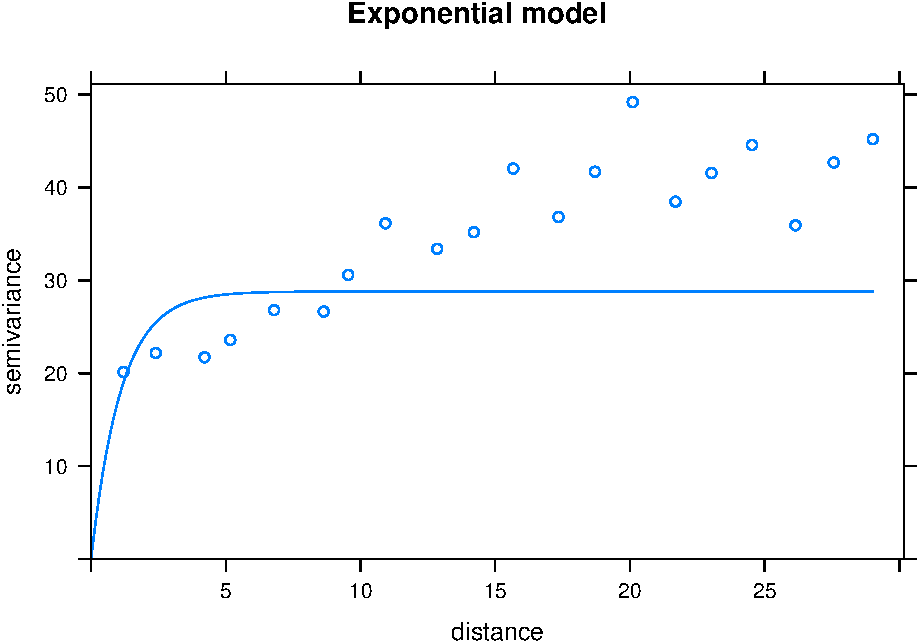
\includegraphics{Field-Trial-Spatial-Analysis-Guide_files/figure-latex/unnamed-chunk-24-1.pdf}

Hmm, that plot is not very convincing.

In this field trial, there is evidence spatial correlation as a function of distance, but there is not evidence that spatial autocorrelation is impacted by the direction.

It's important to remember these methods are intended to describe localised spatial correlation. Field-wide spatial gradients should be modelled as a separate trend.

\hypertarget{ch4}{%
\chapter{Applying Spatial Covariates}\label{ch4}}

\begin{Shaded}
\begin{Highlighting}[]
\KeywordTok{library}\NormalTok{(agridat); }\KeywordTok{library}\NormalTok{(dplyr); }\KeywordTok{library}\NormalTok{(tidyr)}
\KeywordTok{data}\NormalTok{(}\StringTok{"stroup.nin"}\NormalTok{)}

\NormalTok{Nin <-}\StringTok{ }\NormalTok{stroup.nin }\OperatorTok\StringTok{ }\KeywordTok{mutate}\NormalTok{(}\DataTypeTok{col.width =}\NormalTok{ col }\OperatorTok{*}\StringTok{ }\FloatTok{1.2}\NormalTok{, }\DataTypeTok{row.length =}\NormalTok{ row }\OperatorTok{*}\StringTok{ }\FloatTok{4.3}\NormalTok{) }\OperatorTok\StringTok{ }
\StringTok{  }\KeywordTok{mutate}\NormalTok{(}\DataTypeTok{name =} \KeywordTok{case_when}\NormalTok{(}\KeywordTok{is.na}\NormalTok{(}\KeywordTok{as.character}\NormalTok{(rep)) }\OperatorTok{~}\StringTok{ }\OtherTok{NA_character_}\NormalTok{, }
                          \OtherTok{TRUE} \OperatorTok{~}\StringTok{ }\KeywordTok{as.character}\NormalTok{(gen))) }\OperatorTok\StringTok{ }\KeywordTok{arrange}\NormalTok{(col, row) }

\NormalTok{Nin.na <-}\StringTok{ }\KeywordTok{filter}\NormalTok{(Nin, }\OperatorTok{!}\KeywordTok{is.na}\NormalTok{(rep))}

\NormalTok{Nin.spatial <-}\StringTok{ }\NormalTok{Nin.na}
\KeywordTok{coordinates}\NormalTok{(Nin.spatial) <-}\StringTok{ }\ErrorTok{~}\StringTok{ }\NormalTok{col.width }\OperatorTok{+}\StringTok{ }\NormalTok{row.length}
\end{Highlighting}
\end{Shaded}

Once spatial autocorrelation has been identified in field trials, the next logical step is to employ a modelling technique that will reduce the impact of spatial varition on the final estiamtes from the analysis.

\hypertarget{prep-work}{%
\section{Prep work}\label{prep-work}}

As a reminder, the first thing is to run a standard linear model. A common model specification for the randomised complete block design (RCBD) is to include cultivar as a fixed effect and block as a random effect.

Here is the R code for RCBD analsysis of the NIN data set loaded in Section 3 \ref{ch:ch3} that was found to have strong spatial correlation:

\begin{Shaded}
\begin{Highlighting}[]
\KeywordTok{library}\NormalTok{(nlme)}

\NormalTok{nin.lme <-}\StringTok{ }\KeywordTok{lme}\NormalTok{(yield }\OperatorTok{~}\StringTok{ }\NormalTok{gen, }\DataTypeTok{random =} \OperatorTok{~}\DecValTok{1}\OperatorTok{|}\NormalTok{rep,}
              \DataTypeTok{data =}\NormalTok{ Nin,}
              \DataTypeTok{na.action =}\NormalTok{ na.exclude)}

\KeywordTok{anova}\NormalTok{(nin.lme)}
\end{Highlighting}
\end{Shaded}

\begin{verbatim}
##             numDF denDF   F-value p-value
## (Intercept)     1   165 242.05402  <.0001
## gen            55   165   0.87549  0.7119
\end{verbatim}

\begin{Shaded}
\begin{Highlighting}[]
\KeywordTok{library}\NormalTok{(spdep)}
\NormalTok{xy.rook <-}\StringTok{ }\KeywordTok{cell2nb}\NormalTok{(}\DataTypeTok{nrow =} \KeywordTok{max}\NormalTok{(Nin}\OperatorTok{$}\NormalTok{row), }\DataTypeTok{ncol =} \KeywordTok{max}\NormalTok{(Nin}\OperatorTok{$}\NormalTok{col), }\DataTypeTok{type=}\StringTok{"rook"}\NormalTok{) }
\KeywordTok{moran.test}\NormalTok{(}\KeywordTok{residuals}\NormalTok{(nin.lme), }\KeywordTok{nb2listw}\NormalTok{(xy.rook), }\DataTypeTok{na.action =}\NormalTok{ na.exclude)}
\end{Highlighting}
\end{Shaded}

\begin{verbatim}
## 
##  Moran I test under randomisation
## 
## data:  residuals(nin.lme)  
## weights: nb2listw(xy.rook) 
## omitted: 1, 12, 23, 34, 45, 56, 59, 67, 78, 89, 100, 108, 111, 122, 133, 144, 155, 204   
## 
## Moran I statistic standard deviate = 8.1602, p-value < 2.2e-16
## alternative hypothesis: greater
## sample estimates:
## Moran I statistic       Expectation          Variance 
##       0.402504491      -0.004484305       0.002487522
\end{verbatim}

The variables ``gen'' refers to the cultivar or breeding line being trialled, and ``rep'' is the block, and the dependent variable, ``yield'' is grain yield. Basic exploratory analysis was conducted in Section 3 \ref{ch:ch3}.

\hypertarget{correlated-errors-i-spatial-distance}{%
\section{Correlated Errors I: spatial distance}\label{correlated-errors-i-spatial-distance}}

\textbf{Gaussian Example}

In order to fit models using correlated error model, we will need to first obtain preliminary estimates of the nugget, sill and range: from fitting an empirical variogram.

\begin{Shaded}
\begin{Highlighting}[]
\KeywordTok{library}\NormalTok{(gstat)}
\NormalTok{max_dist <-}\StringTok{ }\FloatTok{0.6}\OperatorTok{*}\KeywordTok{max}\NormalTok{(}\KeywordTok{dist}\NormalTok{(}\KeywordTok{coordinates}\NormalTok{(Nin.spatial)))}
\NormalTok{resid.var1 <-}\StringTok{ }\KeywordTok{variogram}\NormalTok{(yield }\OperatorTok{~}\StringTok{ }\NormalTok{rep }\OperatorTok{+}\StringTok{ }\NormalTok{gen, }
                        \DataTypeTok{cutoff =}\NormalTok{ max_dist,}
                        \DataTypeTok{width =}\NormalTok{ max_dist}\OperatorTok{/}\DecValTok{29}\NormalTok{, }
                        \DataTypeTok{data =}\NormalTok{ Nin.spatial)}
\NormalTok{nugget_start <-}\StringTok{ }\KeywordTok{min}\NormalTok{(resid.var1}\OperatorTok{$}\NormalTok{gamma)}
\end{Highlighting}
\end{Shaded}

\begin{verbatim}

Nin.vgm1 <- vgm(model = "Exp", nugget = nugget_start) 
Nin.vgm2 <- vgm(model = "Sph", nugget = nugget_start) 

Nin.vgm4 <- vgm(model = "Mat", nugget = nugget_start)

Nin.variofit1 <- fit.variogram(resid.var1, Nin.vgm1)
Nin.variofit2 <- fit.variogram(resid.var1, Nin.vgm2)

Nin.variofit4 <- fit.variogram(resid.var1, Nin.vgm4)
\end{verbatim}

In the previous section, an isotropic Gaussian function was identified as the best mocel for describing the decay of eror correlation over distance.

\begin{Shaded}
\begin{Highlighting}[]
\NormalTok{Nin.vgm <-}\StringTok{ }\KeywordTok{vgm}\NormalTok{(}\DataTypeTok{model =} \StringTok{"Gau"}\NormalTok{, }\DataTypeTok{nugget =}\NormalTok{ nugget_start) }
\NormalTok{Nin.variofit <-}\StringTok{ }\KeywordTok{fit.variogram}\NormalTok{(resid.var1, Nin.vgm)}

\NormalTok{nugget <-}\StringTok{ }\NormalTok{Nin.variofit}\OperatorTok{$}\NormalTok{psill[}\DecValTok{1}\NormalTok{] }
\NormalTok{range <-}\StringTok{ }\NormalTok{Nin.variofit}\OperatorTok{$}\NormalTok{range[}\DecValTok{2}\NormalTok{] }
\NormalTok{sill <-}\StringTok{ }\KeywordTok{sum}\NormalTok{(Nin.variofit}\OperatorTok{$}\NormalTok{psill) }
\NormalTok{nugget.effect <-}\StringTok{  }\NormalTok{nugget}\OperatorTok{/}\NormalTok{sill}
\end{Highlighting}
\end{Shaded}

Next, create a correlated error structure (from the \textbf{nlme} package).

\begin{Shaded}
\begin{Highlighting}[]
\NormalTok{cor.gaus <-}\StringTok{ }\KeywordTok{corSpatial}\NormalTok{(}\DataTypeTok{value =} \KeywordTok{c}\NormalTok{(range, nugget.effect), }
                  \DataTypeTok{form =} \OperatorTok{~}\StringTok{ }\NormalTok{row.length }\OperatorTok{+}\StringTok{ }\NormalTok{col.width, }
                  \DataTypeTok{nugget =}\NormalTok{ T, }\DataTypeTok{fixed =}\NormalTok{ F,}
                  \DataTypeTok{type =} \StringTok{"gaussian"}\NormalTok{, }
                  \DataTypeTok{metric =} \StringTok{"euclidean"}\NormalTok{)}
\end{Highlighting}
\end{Shaded}

Last, update the linear mixed model with the correlated error strucutre and inspect the results:

\begin{Shaded}
\begin{Highlighting}[]
\NormalTok{nin.gaus <-}\StringTok{ }\KeywordTok{update}\NormalTok{(nin.lme, }\DataTypeTok{corr =}\NormalTok{ cor.gaus)}
\KeywordTok{anova}\NormalTok{(nin.gaus)}
\end{Highlighting}
\end{Shaded}

\begin{verbatim}
##             numDF denDF   F-value p-value
## (Intercept)     1   165 157.36740  <.0001
## gen            55   165   1.78151  0.0028
\end{verbatim}

\begin{Shaded}
\begin{Highlighting}[]
\CommentTok{#moran.test(residuals(nin.gaus), nb2listw(xy.rook), na.action = na.exclude)}
\end{Highlighting}
\end{Shaded}

Other models can be implemented quite similarily:

\hypertarget{exponential}{%
\subsection{Exponential}\label{exponential}}

\begin{Shaded}
\begin{Highlighting}[]
\KeywordTok{rm}\NormalTok{(Nin.vgm, Nin.variofit, nugget, sill, range, nugget.effect)}

\NormalTok{Nin.vgm <-}\StringTok{ }\KeywordTok{vgm}\NormalTok{(}\DataTypeTok{model =} \StringTok{"Exp"}\NormalTok{, }\DataTypeTok{nugget =}\NormalTok{ nugget_start) }
\NormalTok{Nin.variofit <-}\StringTok{ }\KeywordTok{fit.variogram}\NormalTok{(resid.var1, Nin.vgm)}

\NormalTok{nugget <-}\StringTok{ }\NormalTok{Nin.variofit}\OperatorTok{$}\NormalTok{psill[}\DecValTok{1}\NormalTok{] }
\NormalTok{range <-}\StringTok{ }\NormalTok{Nin.variofit}\OperatorTok{$}\NormalTok{range[}\DecValTok{2}\NormalTok{] }
\NormalTok{sill <-}\StringTok{ }\KeywordTok{sum}\NormalTok{(Nin.variofit}\OperatorTok{$}\NormalTok{psill) }
\NormalTok{nugget.effect <-}\StringTok{  }\NormalTok{nugget}\OperatorTok{/}\NormalTok{sill}

\NormalTok{cor.exp <-}\StringTok{ }\KeywordTok{corSpatial}\NormalTok{(}\DataTypeTok{value =} \KeywordTok{c}\NormalTok{(range, nugget.effect), }
                  \DataTypeTok{form =} \OperatorTok{~}\StringTok{ }\NormalTok{row.length }\OperatorTok{+}\StringTok{ }\NormalTok{col.width, }
                  \DataTypeTok{nugget =}\NormalTok{ T, }\DataTypeTok{fixed =}\NormalTok{ F,}
                  \DataTypeTok{type =} \StringTok{"exponential"}\NormalTok{, }
                  \DataTypeTok{metric =} \StringTok{"euclidean"}\NormalTok{)}

\NormalTok{nin.exp <-}\StringTok{ }\KeywordTok{update}\NormalTok{(nin.lme, }\DataTypeTok{corr =}\NormalTok{ cor.exp)}
\KeywordTok{anova}\NormalTok{(nin.exp)}
\end{Highlighting}
\end{Shaded}

\begin{verbatim}
##             numDF denDF  F-value p-value
## (Intercept)     1   165 62.35102  <.0001
## gen            55   165  1.83489  0.0018
\end{verbatim}

\hypertarget{spherical}{%
\subsection{Spherical}\label{spherical}}

\begin{Shaded}
\begin{Highlighting}[]
\KeywordTok{rm}\NormalTok{(Nin.vgm, Nin.variofit, nugget, sill, range, nugget.effect)}

\NormalTok{Nin.vgm <-}\StringTok{ }\KeywordTok{vgm}\NormalTok{(}\DataTypeTok{model =} \StringTok{"Sph"}\NormalTok{, }\DataTypeTok{nugget =}\NormalTok{ nugget_start) }
\NormalTok{Nin.variofit <-}\StringTok{ }\KeywordTok{fit.variogram}\NormalTok{(resid.var1, Nin.vgm)}

\NormalTok{nugget <-}\StringTok{ }\NormalTok{Nin.variofit}\OperatorTok{$}\NormalTok{psill[}\DecValTok{1}\NormalTok{] }
\NormalTok{range <-}\StringTok{ }\NormalTok{Nin.variofit}\OperatorTok{$}\NormalTok{range[}\DecValTok{2}\NormalTok{] }
\NormalTok{sill <-}\StringTok{ }\KeywordTok{sum}\NormalTok{(Nin.variofit}\OperatorTok{$}\NormalTok{psill) }
\NormalTok{nugget.effect <-}\StringTok{  }\NormalTok{nugget}\OperatorTok{/}\NormalTok{sill}

\NormalTok{cor.sph <-}\StringTok{ }\KeywordTok{corSpatial}\NormalTok{(}\DataTypeTok{value =} \KeywordTok{c}\NormalTok{(range, nugget.effect), }
                  \DataTypeTok{form =} \OperatorTok{~}\StringTok{ }\NormalTok{row.length }\OperatorTok{+}\StringTok{ }\NormalTok{col.width, }
                  \DataTypeTok{nugget =}\NormalTok{ T, }\DataTypeTok{fixed =}\NormalTok{ F,}
                  \DataTypeTok{type =} \StringTok{"spherical"}\NormalTok{, }
                  \DataTypeTok{metric =} \StringTok{"euclidean"}\NormalTok{)}

\NormalTok{nin.sph <-}\StringTok{ }\KeywordTok{update}\NormalTok{(nin.lme, }\DataTypeTok{corr =}\NormalTok{ cor.sph)}
\KeywordTok{anova}\NormalTok{(nin.sph)}
\end{Highlighting}
\end{Shaded}

\begin{verbatim}
##             numDF denDF   F-value p-value
## (Intercept)     1   165 121.43563  <.0001
## gen            55   165   1.83709  0.0018
\end{verbatim}

\hypertarget{power}{%
\subsection{Power}\label{power}}

\begin{Shaded}
\begin{Highlighting}[]
\KeywordTok{rm}\NormalTok{(Nin.vgm, Nin.variofit, nugget, sill, range, nugget.effect)}

\NormalTok{cor.pow <-}\StringTok{ }\KeywordTok{corSpatial}\NormalTok{(}\DataTypeTok{form =} \OperatorTok{~}\StringTok{ }\NormalTok{row.length }\OperatorTok{+}\StringTok{ }\NormalTok{col.width, }
                  \DataTypeTok{nugget =}\NormalTok{ T, }\DataTypeTok{fixed =}\NormalTok{ F,}
                  \DataTypeTok{type =} \StringTok{"ratio"}\NormalTok{, }
                  \DataTypeTok{metric =} \StringTok{"euclidean"}\NormalTok{)}

\NormalTok{nin.pow <-}\StringTok{ }\KeywordTok{update}\NormalTok{(nin.lme, }\DataTypeTok{corr =}\NormalTok{ cor.pow)}
\KeywordTok{anova}\NormalTok{(nin.pow)}
\end{Highlighting}
\end{Shaded}

\begin{verbatim}
##             numDF denDF  F-value p-value
## (Intercept)     1   165 78.54890  <.0001
## gen            55   165  1.78787  0.0027
\end{verbatim}

In the **nlme* package, there is also an option for a linear model in the \texttt{corSpatial()} function. However, it is recommended that a linear trend be fitted to the data instead.

The package **spaMM* implements additional correlation models such as Matérn, Cauchy and more.

\hypertarget{nearest-neighbor-approaches-1}{%
\section{Nearest Neighbor Approaches}\label{nearest-neighbor-approaches-1}}

\hypertarget{estimating-lagged-autocorrelation}{%
\subsection{estimating lagged autocorrelation}\label{estimating-lagged-autocorrelation}}

Prior to running any nearest neighbor appraoches, it is helpful to understand the lagged spatial autocorrelation.

\hypertarget{durban}{%
\subsection{Durban}\label{durban}}

??

\hypertarget{spatial-lag-model}{%
\subsection{Spatial lag model}\label{spatial-lag-model}}

\begin{Shaded}
\begin{Highlighting}[]
\KeywordTok{library}\NormalTok{(spatialreg)}

\NormalTok{nin.lag <-}\StringTok{ }\KeywordTok{lagsarlm}\NormalTok{(yield }\OperatorTok{~}\StringTok{ }\NormalTok{gen }\OperatorTok{+}\StringTok{ }\NormalTok{rep,}
                       \DataTypeTok{listw =} \KeywordTok{nb2listw}\NormalTok{(xy.rook),}
                       \DataTypeTok{data =}\NormalTok{ Nin, }\DataTypeTok{na.action =}\NormalTok{ na.exclude)}

\KeywordTok{moran.mc}\NormalTok{(}\KeywordTok{residuals}\NormalTok{(nin.lag), }\KeywordTok{nb2listw}\NormalTok{(xy.rook), }\DecValTok{999}\NormalTok{, }\DataTypeTok{na.action =}\NormalTok{ na.exclude)}
\end{Highlighting}
\end{Shaded}

\begin{verbatim}
## 
##  Monte-Carlo simulation of Moran I
## 
## data:  residuals(nin.lag) 
## weights: nb2listw(xy.rook) 
## omitted: 1, 12, 23, 34, 45, 56, 59, 67, 78, 89, 100, 108, 111, 122, 133, 144, 155, 204 
## number of simulations + 1: 1000 
## 
## statistic = -0.080738, observed rank = 49, p-value = 0.951
## alternative hypothesis: greater
\end{verbatim}

\hypertarget{spatial-error-model}{%
\subsection{Spatial error model}\label{spatial-error-model}}

\begin{Shaded}
\begin{Highlighting}[]
\NormalTok{nin.sem <-}\StringTok{ }\KeywordTok{errorsarlm}\NormalTok{(yield }\OperatorTok{~}\StringTok{ }\NormalTok{gen }\OperatorTok{+}\StringTok{ }\NormalTok{rep,}
                       \DataTypeTok{listw =} \KeywordTok{nb2listw}\NormalTok{(xy.rook),}
                       \DataTypeTok{data =}\NormalTok{ Nin, }\DataTypeTok{na.action =}\NormalTok{ na.exclude)}

\KeywordTok{moran.mc}\NormalTok{(}\KeywordTok{residuals}\NormalTok{(nin.sem), }\KeywordTok{nb2listw}\NormalTok{(xy.rook), }\DecValTok{999}\NormalTok{, }\DataTypeTok{na.action =}\NormalTok{ na.exclude)}
\end{Highlighting}
\end{Shaded}

\begin{verbatim}
## 
##  Monte-Carlo simulation of Moran I
## 
## data:  residuals(nin.sem) 
## weights: nb2listw(xy.rook) 
## omitted: 1, 12, 23, 34, 45, 56, 59, 67, 78, 89, 100, 108, 111, 122, 133, 144, 155, 204 
## number of simulations + 1: 1000 
## 
## statistic = -0.1144, observed rank = 13, p-value = 0.987
## alternative hypothesis: greater
\end{verbatim}

\hypertarget{combined-spatial-lag-and-error-model-arma}{%
\subsection{Combined spatial lag and error model (ARMA)}\label{combined-spatial-lag-and-error-model-arma}}

\begin{Shaded}
\begin{Highlighting}[]
\NormalTok{nin.arma <-}\StringTok{ }\KeywordTok{sacsarlm}\NormalTok{(yield }\OperatorTok{~}\StringTok{ }\NormalTok{gen }\OperatorTok{+}\StringTok{ }\NormalTok{rep,}
                       \DataTypeTok{listw =} \KeywordTok{nb2listw}\NormalTok{(xy.rook),}
                       \DataTypeTok{data =}\NormalTok{ Nin, }\DataTypeTok{na.action =}\NormalTok{ na.exclude)}

\KeywordTok{moran.mc}\NormalTok{(}\KeywordTok{residuals}\NormalTok{(nin.arma), }\KeywordTok{nb2listw}\NormalTok{(xy.rook), }\DecValTok{999}\NormalTok{, }\DataTypeTok{na.action =}\NormalTok{ na.exclude)}
\end{Highlighting}
\end{Shaded}

\begin{verbatim}
## 
##  Monte-Carlo simulation of Moran I
## 
## data:  residuals(nin.arma) 
## weights: nb2listw(xy.rook) 
## omitted: 1, 12, 23, 34, 45, 56, 59, 67, 78, 89, 100, 108, 111, 122, 133, 144, 155, 204 
## number of simulations + 1: 1000 
## 
## statistic = -0.036476, observed rank = 250, p-value = 0.75
## alternative hypothesis: greater
\end{verbatim}

\hypertarget{p-splines}{%
\section{p-Splines}\label{p-splines}}

\hypertarget{ar1xar1-not-possible}{%
\subsection{AR1xAR1 (not possible!!)}\label{ar1xar1-not-possible}}

\hypertarget{ch3-part3}{%
\chapter{Comparing Spatial Models}\label{ch3-part3}}

\hypertarget{example-one}{%
\section{Example one}\label{example-one}}

\hypertarget{example-two}{%
\section{Example two}\label{example-two}}

\bibliography{book.bib,packages.bib}


\end{document}
